\documentclass[10pt, conference]{IEEEtran}
\IEEEoverridecommandlockouts
% The preceding line is only needed to identify funding in the first footnote. If that is unneeded, please comment it out.
\usepackage{cite}
\usepackage{amsmath,amssymb,amsfonts}
\usepackage{algorithm}
\usepackage{algorithmic}
\usepackage{graphicx}
\usepackage{textcomp}
\usepackage{xcolor}
\usepackage{multirow}
\usepackage{tablefootnote}
\usepackage{xspace}

\def\BibTeX{{\rm B\kern-.05em{\sc i\kern-.025em b}\kern-.08em
    T\kern-.1667em\lower.7ex\hbox{E}\kern-.125emX}}

\newcommand{\sysname}{MAGIC\xspace}
\newcommand{\revision}[1]{\textcolor{red}{#1}}

\begin{document}

\title{Classifying Malware Represented as Control Flow Graphs using Deep Graph Convolutional Neural Network}

\author{
\IEEEauthorblockN{Jiaqi Yan}
\IEEEauthorblockA{Illinois Institute of Technology \\
jyan31@hawk.iit.edu}
\and
\IEEEauthorblockN{Guanhua Yan}
\IEEEauthorblockA{Binghamton University, State University of New York \\
ghyan@binghamton.edu}
\and
\IEEEauthorblockN{Dong Jin}
\IEEEauthorblockA{Illinois Institute of Technology  \\
dong.jin@iit.edu}
% \IEEEauthorblockN{Kyon Jon Smith, Yuki Nagato, Haruhi Suzumiya}
% \IEEEauthorblockA{\textit{SOS Brigade}  \\
% \textit{Kitakou North High} \\
% Nishinomiya, JP \\
% \{kyon.jsmith, yuki.nagato, iamgod\}@sos.knh.jp}
}

\maketitle

\begin{abstract}
\if 0
Malware remains one of the biggest cyber threats in the modern digital world.
Existing machine-learning-based malware classification approaches highly rely on non-intuitive and non-generic engineered features extracted from binary bytes or assembly code.
This paper proposes a malware detection and classification method featuring several unique advantages.
We represent binary executable as a \textit{Control Flow Graph} (CFG), which fully preserves the logic of the program.
Within CFG, we can freely extract both instruction-level and vertex-to-vertex attributes from each code block,
and then build an \textit{Attributed Control Flow Graph} (ACFG), a generic format for arbitrary binaries.
However, the existing works of malware analysis using ACFG have to rely on inefficient and inadaptive graph matching techniques.
To overcome the drawbacks, we propose to use the \textit{Deep Graph Convolutional Neural Network} (DGCNN) to fuse the vertices attributes of the graph structure in a breadth-first-search fashion.
Learning informative hidden features and training classifier are performed together by minimizing the malware classification error.
We transform two independent datasets into the generic ACFG format, and conduct evaluation over totaling 20K ACFG samples.
The results show that our deep convolution model effectively detects malware represented as ACFG,
and achieves competitive performance comparing to the state-of-the-art methods.
\fi 
Malware have been one of the biggest cyber threats in the digital world for a long time.
Existing machine learning-based malware classification methods rely on handcrafted features extracted from raw binary files or disassembled code.
The diversity of such features created has made it hard to build generic malware classification systems that
work effectively across different operational environments.
To strike a balance between generality and performance,
we explore new machine learning techniques to classify malware programs represented as their control flow graphs (CFGs).
To overcome the drawbacks of existing malware analysis methods using inefficient and non-adaptive graph matching techniques, in this work,
we build a new system that uses deep graph convolutional neural network to embed structural information inherent in CFGs for effective yet efficient malware classification.
We use two large independent datasets that contain more than 20K malware samples to evaluate our proposed system and
the experimental results show that it can classify CFG-represented malware programs with performance
comparable to those of the state-of-the-art methods applied on handcrafted malware features.

\end{abstract}

\begin{IEEEkeywords}
malware classification, control flow graph, deep learning, graph convolution
\end{IEEEkeywords}

\Section{Deep Learning Based Cyber Security System}
\label{DL:Sec:Intro}

Deep learning has gained a dramatic increase in popularity in the last couple of years,
and has offered advanced solutions in the areas of image and speech recognition~\cite{AlexNet, SpeechDNN},
natural language processing~\cite{Word2Vec}, Go playing~\cite{AlphaGo}, and many other domains~\cite{DeepLearning}. 
Motivated by deep learning's success, we ask what deep learning technology can do for cyber security.
Specifically, we focus on the domain of intrusion detection system.
Though both motivated by the deep learning technology, we have different answers for network-based and host-based intrusion detection systems respectively.


\Subsection{Deep Learning Based Network Intrusion Detection System}
\label{DL:SubSec:NIDS}
As networking technology gets deeply integrated into our lives, protecting modern networked systems against cyber-attacks is no longer optional.
Network intrusion detection systems (NIDSes) are essential security solutions for today's networked systems supporting military applications,
social communications, cloud services, and other critical infrastructures.
A NIDS automatically monitors traffic in a network to detect malicious activities and policy violations.
The majority of NIDSes today adopt signature-based detection techniques,
which can only identify known attacks via matching pre-installed signatures to observed network activities. 
The signature databases have to be frequently updated to include new types of attacks.
Those limitations have motivated researchers to investigate anomaly detection based approaches~\cite{STL-NIDS, LOF, RankingOutliner, NB-Tree, RampLossKSVCR, GAA-ADS}. 

Anomaly detection approaches use data mining or machine learning techniques to mathematically model the trustworthy network activities based on a set of training data,
and detect deviations from the model in observed data. A key advantage is the ability to detect unknown or novel malicious activities.
An on-line model further frees network administrators from identifying new patterns or even new types of the abnormal behaviors in a dynamic network environment.
However, if the constructed model is not sufficiently generalized for normal or abnormal traffic,
anomaly-based approaches would suffer from high false positive, i.e., incorrectly treat unknown normal traffic as malicious.

We study the feasibility of off-line deep learning based NIDS by constructing the detection engine with
multiple advanced deep learning models and conducting a quantitative and comparative evaluation of those models.
Specifically, we first introduce the general deep learning methodology and its potential implication on the network intrusion detection problem.
We then review multiple machine learning solutions to two network intrusion detection tasks (NSL-KDD and UNSW-NB15 datasets).
We develop a TensorFlow-based deep learning library, called NetLearner, and implement a handful of cutting-edge deep learning models for NIDS.
Finally, we conduct a quantitative and comparative performance evaluation of those models using NetLearner.


\section{System Overview of \sysname}
\label{MG:Sec:System}

%Before that, let's take an overview of the components in \sysname in the pipeline order.
This section overviews the three main components of \sysname, whose workflow is illustrated in Figure~\ref{fig:SystemPipeline}.

\begin{figure*}[htbp]
\centerline{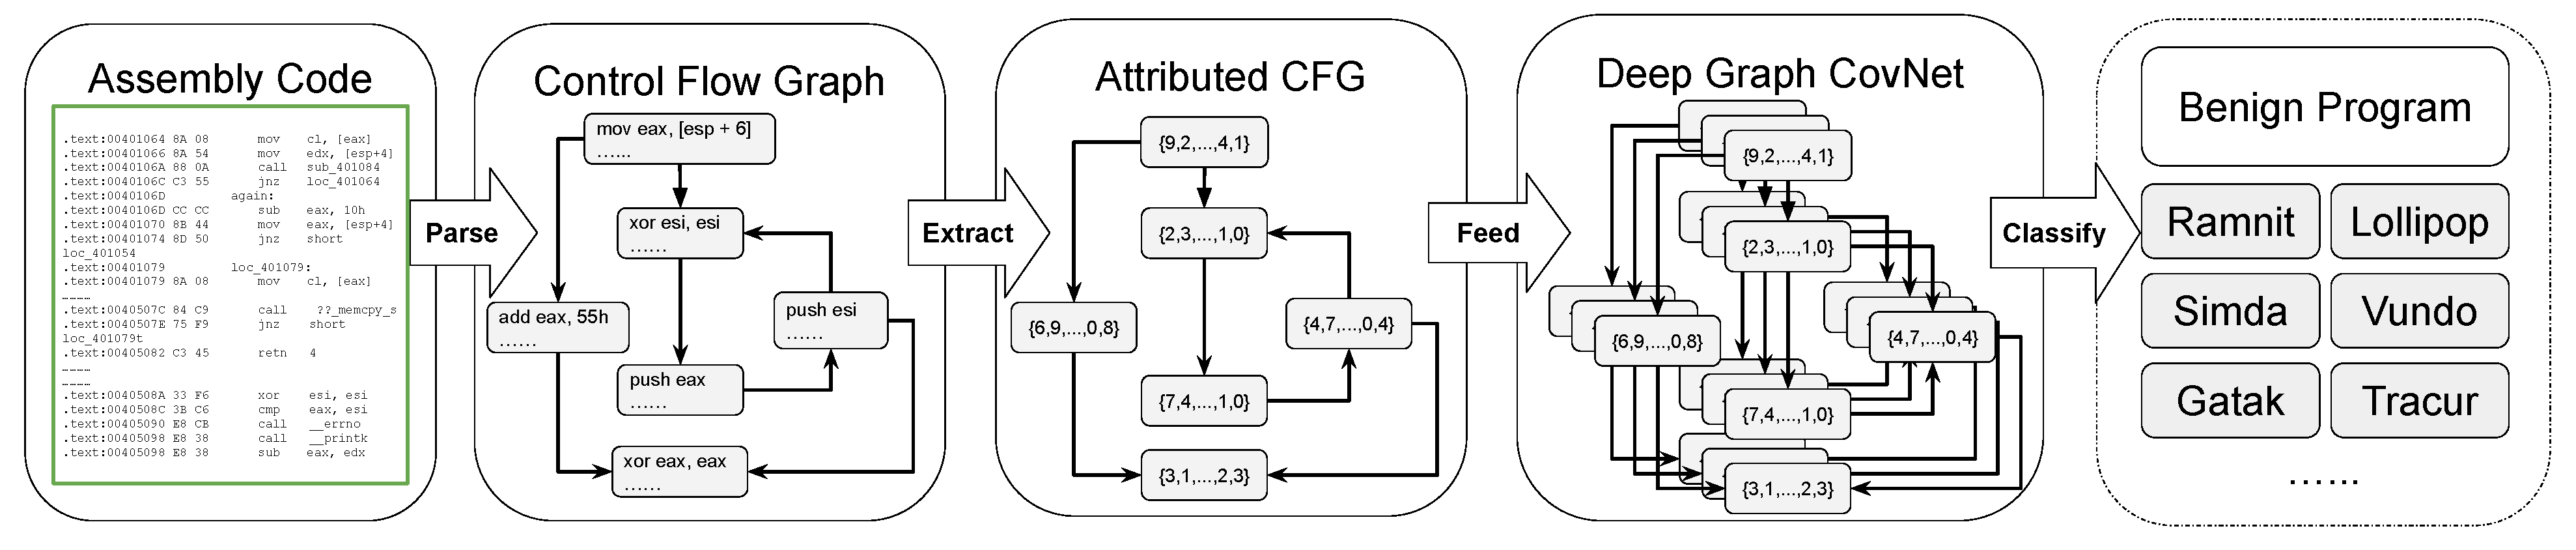
\includegraphics[width=1.0\textwidth]{Magic/figures/SystemPipeline.eps}}
\caption{The workflow of \sysname, a DGCNN-based malware classification system}
\label{fig:SystemPipeline}
\end{figure*}

\subsection{Control Flow Graph}\label{subsec:ConstructCfg}
%Given a cross-platform assembly code, 

\sysname relies on the state-of-the-art tools, such as IDA Pro~\cite{bib:idapro}, to extract CFGs from malware code.
In a CFG, a vertex represents a basic block, which contains a straight sequence of code or assembly instructions without any control flow transition except at its exit.
Two vertices $(u, v)$ are connected by a directed edge $u \rightarrow v$ if either the last instruction in $u$ falls through the first line of code in $v$,
or there is a jump instruction in $u$ that is destined to some instructions (e.g., jump target) in $v$.
The implementation details on how to build the CFG from disassembled execution code will be given in Section~\ref{sec:BuildCfg}.

\subsection{Attributed Control Flow Graph}\label{subsec:Cfg2Acfg}
The CFG representation of software program is generic for the purpose of malware classification in several ways.
First, this type of representation transcends specific programming languages in which the programs are written or hardware platforms for which the programs are developed.
Although other low-level representations such as hexadecimal byte sequences have similar properties, a CFG explicitly expresses the execution logic of a program using a graph data structure.
Hence, the semantics of a malware program is embodied by not only the characteristics of the code in individual basic blocks but also their structural dependencies defined by the edges connecting these basic blocks. 


%which can be used as raw features us works on ML-based malware classification but also 

%The expressive power of CFGs also enables the collection of a variety of aggregate features


%Furthermore, the vertices in the graph provide us a suitable unit environment to extract code-level attributes, many of which are scatteringly adopted by existing machine learning models as raw features.

To convert CFGs to structures that are amenable to machine learning, we define attributes at each vertex that summarize code characteristics as numerical values.
Initially the attributes computed at a vertex do not contain any structural information, which means that their values are independently collected from the corresponding basic block.
Table~\ref{tab:UsedAttributes} lists the attributes implemented in our prototype system, although more attributes can be conveniently added to further improve malware classification performance.

\begin{table}[htbp]
\caption{Block-level attributes used in \sysname}
\begin{center}
\begin{tabular}{c|l}
\hline
Attribute Type & Attribute Description \\
\hline
\multirow{10}{*}{From Code Sequence} & \# Numeric Constants \\
 & \# Transfer Instructions         \\
 & \# Call Instructions             \\
 & \# Arithmetic Instructions       \\
 & \# Compare Instructions          \\
% & \# Crypto instructions           \\
 & \# Mov Instructions              \\
 & \# Termination Instructions      \\
 & \# Data Declaration Instructions \\
 & \# Total Instructions            \\
\hline
\multirow{2}{*}{From Vertex Structure} & \# Offspring, i.e., Degree \\
 & \# Instructions in the Vertex    \\
 \hline
\end{tabular}
\label{tab:UsedAttributes}
\end{center}
\end{table}

As the raw attributes in an attributed CFG (ACFG) contain little structural information and the number of vertices in an ACFG varies with the individual program from which the CFG is derived, for the purpose of malware classification it is necessary to aggregate these attributes over all the vertices in the ACFG in an organic manner depending on its graph structure.
The task of such attribute aggregation is accomplished with DGCNN, which shall be explained next.

%Figure~\ref{fig:SystemPipeline} shows how the further processing on the vertices of a CFG offers us the attributed CFG representation.

%Attributes are numeric values that characterize a vertex in a CFG.
%It usually describes the sequence of code inside a code block, such as the number of constants and the number of transfer instructions.
%It also includes structural information of the vertex, such as the number of offspring and betweenness.


\subsection{Deep Graph Convolution Neural Network}\label{subsec:DGCNN}
Unlike image or text-based data, graph-based data are of variable sizes and are thus not naturally ordered tensors.
%Therefore, a gap exists between the ACFG and the optimal features on the basis of which a machine-learning-powered detection engine makes malware prediction. In our pipeline, this gap is bridged by 
To address this challenge, we use the state-of-the-art deep neural network that can automatically learn discriminative latent features from malware data abstracted as ACFGs.
Particularly, we use deep graph convolution neural network to transform unordered graph data of varying sizes to tensors of fixed size and order.
The transformation algorithm first recursively propagates the weighted attributes in each vertex through the neighborhood defined by the graph structure.
Next, it sorts the vertices in the order of their feature descriptors.
After the sorting step, the graphs with variant sizes are embedded into fixed-size vectors, which are amenable to ML-based classification.
In the next section, we shall elaborate on these operations as well as our extensions based on formal mathematical descriptions.

\section{Algorithm Description}
\label{MG:Sec:DGCNN}

Our work on applying DGCNN for malware classification in \sysname has been inspired by the deep learning model proposed in~\cite{Dgcnn}. In this section, we first introduce how DGCNN aggregates attributes through the neighborhood defined by the graph structure. We then discuss how to extend the existing DGCNN model with our own modifications. To explain the rationale of the DGCNN-based malware classification algorithm clearly, we walk through an example graph with five vertices as shown in Figure~\ref{MG:Fig:ExampleGraph}.

\subsection{Primer on DGCNN}

\textbf{Notations.} We denote the adjacency matrix of a graph $G=(V, E)$ of $n$ vertices as $\mathbf{A} \in \mathbb{Z} ^{n\times n}$.
Note that $G$ is a directed graph, and $\mathbf{A}$ is not necessarily symmetric.
To allow the attributes of a vertex to be propagated back to the vertex itself, we define the augmented adjacency matrix $\tilde{\mathbf{A}} = \mathbf{A} + \mathbf{I}$.
Accordingly, the augmented diagonal degree matrix of $G$ is defined as $\tilde{\mathbf{D}}$, where
$\tilde{\mathbf{D}}_{i,i} = \sum_j \tilde{\mathbf{A}}_{i,j}$.
We assume that each vertex is associated with a $c$-dimension attribute vector.
Therefore, we use $\mathbf{X} \in \mathbb{R}^{n \times c}$ to denote the attribute matrix for all the vertices in the graph. %$\forall v \in V$.
Alternatively, we can also treat $\mathbf{X}$ as the concatenation of $c$ \textit{attribute channels} of the graph.
For the sample graph $g$ in Figure~\ref{MG:Fig:ExampleGraph}, we assume the vertices have two attribute channels,
and display the corresponding augmented adjacency matrix $\tilde{\mathbf{A}}$, the augmented diagonal degree matrix $\tilde{\mathbf{D}}$,
and the attribute matrix $\mathbf{X}$ with two attribute channels named $F1$ and $F2$.
Given $\tilde{\mathbf{A}}$ and $\mathbf{X}$ for graph $G$, the DGCNN-based algorithm performs three sequential stages to obtain its tensor representation for malware classification. Note that $\tilde{\mathbf{D}}$ can be calculated from $\tilde{\mathbf{A}}$.

\begin{figure*}[htbp]
\centerline{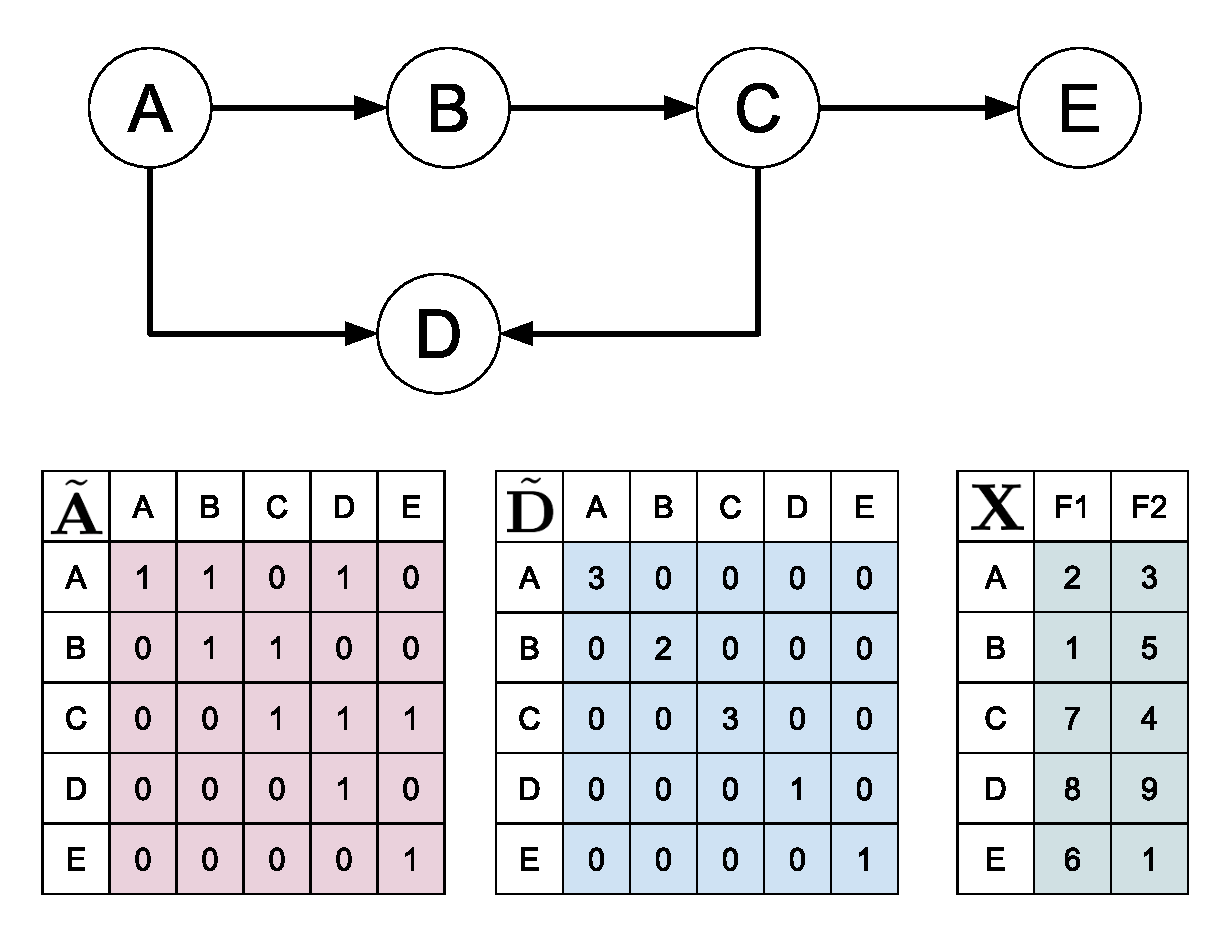
\includegraphics[width=0.90\textwidth]{Magic/figures/ExampleGraph.eps}}
\caption{An Example Graph $g$ and its Corresponding Matrices.}
\label{MG:Fig:ExampleGraph}
\end{figure*}

\textbf{Graph Convolution Layer(s).} In the first stage, a \textit{graph convolution} technique propagates each vertex's attributes to its neighborhood based on the structural connectivity.
To aggregate multi-scale sub-structural attributes, multiple graph
convolution layers are stacked, which can be defined recursively as follows:
\begin{equation}
    \mathbf{Z}^{t + 1} = f(\tilde{\mathbf{D}}^{-1} \tilde{\mathbf{A}} \mathbf{Z}^t \mathbf{W}^t)
\end{equation}
where $Z^0 = X$. The $t$-th layer takes input $Z^t \in \mathbb{Z}^{n \times c_t}$,
mapping $c_t$ feature channels into $c_{t+1}$ feature channels with the graph convolution parameter $\mathbf{W}^t \in \mathbb{R}^{c_t \times c_{t+1}}$.
The newly obtained channels of each vertex are then propagated to both its neighboring vertices and itself,
 first multiplied with the augmented adjacency matrix $\tilde{\mathbf{A}}$,
and then normalized row-wisely using the augmented degree diagonal matrix $\tilde{\mathbf{D}}$.
This key step enables vertices to pass its own attributes through the graph in a breadth-first-search fashion. %It can be explained as follows.
Define $\mathbf{F} = \mathbf{Z}^t \cdot \mathbf{W}^t$ and $\mathbf{O} = \tilde{\mathbf{A}} \cdot \mathbf{F}$, where
\begin{align}
    \mathbf{O}[i][j] &= \sum_{k = 1}^{n} \tilde{\mathbf{A}}[i][k] \times \mathbf{F}[k][j]
\end{align}
$\forall 1\leq i \leq n, 1 \leq j \leq c_t$.
In other words, the $j$-th feature channel of vertex $i$ is computed as a linear combination of all its neighbors' $j$-th feature channels.
The layer finally outputs the element-wise activation using a nonlinear function $f$.
At the end of $h$ graph convolution layers, DGCNN concatenates each layer's output $Z^{t}$,
denoted as $\mathbf{Z}^{1:h} = [\mathbf{Z}^1, \mathbf{Z}^2, \ldots, \mathbf{Z}^{h}]$.
For the sample graph $g$, Figure~\ref{MG:Fig:ExampleGraphConvolution} shows how the two sequential graph convolution layers transform the initial attribute matrix $\mathbf{Z}_0=\mathbf{X}$ to $\mathbf{Z}_1$ and $\mathbf{Z}_2$, both of which together form $\mathbf{Z}^{1:2}$.
After applying $h=2$ graph convolution layers, the sample graph $g$ is transformed to $\mathbf{Z}^{1:h}$.
We assume the weight parameters in the two graph convolution layers are $\mathbf{W}^1 = [[1, 0 ,1], [0, 1, 0]]$ and $\mathbf{W}^2 = [[0, 1 ,-2, 2], [1, 1, 7, -2], [1, 0, -1, 4]]$.
For simplicity, numbers are of 2 precision, and we perform the element-wise RELU nonlinear activation $f(x) = max(x, 0)$ in both graph convolution layers.

\begin{figure*}[htbp]
\centerline{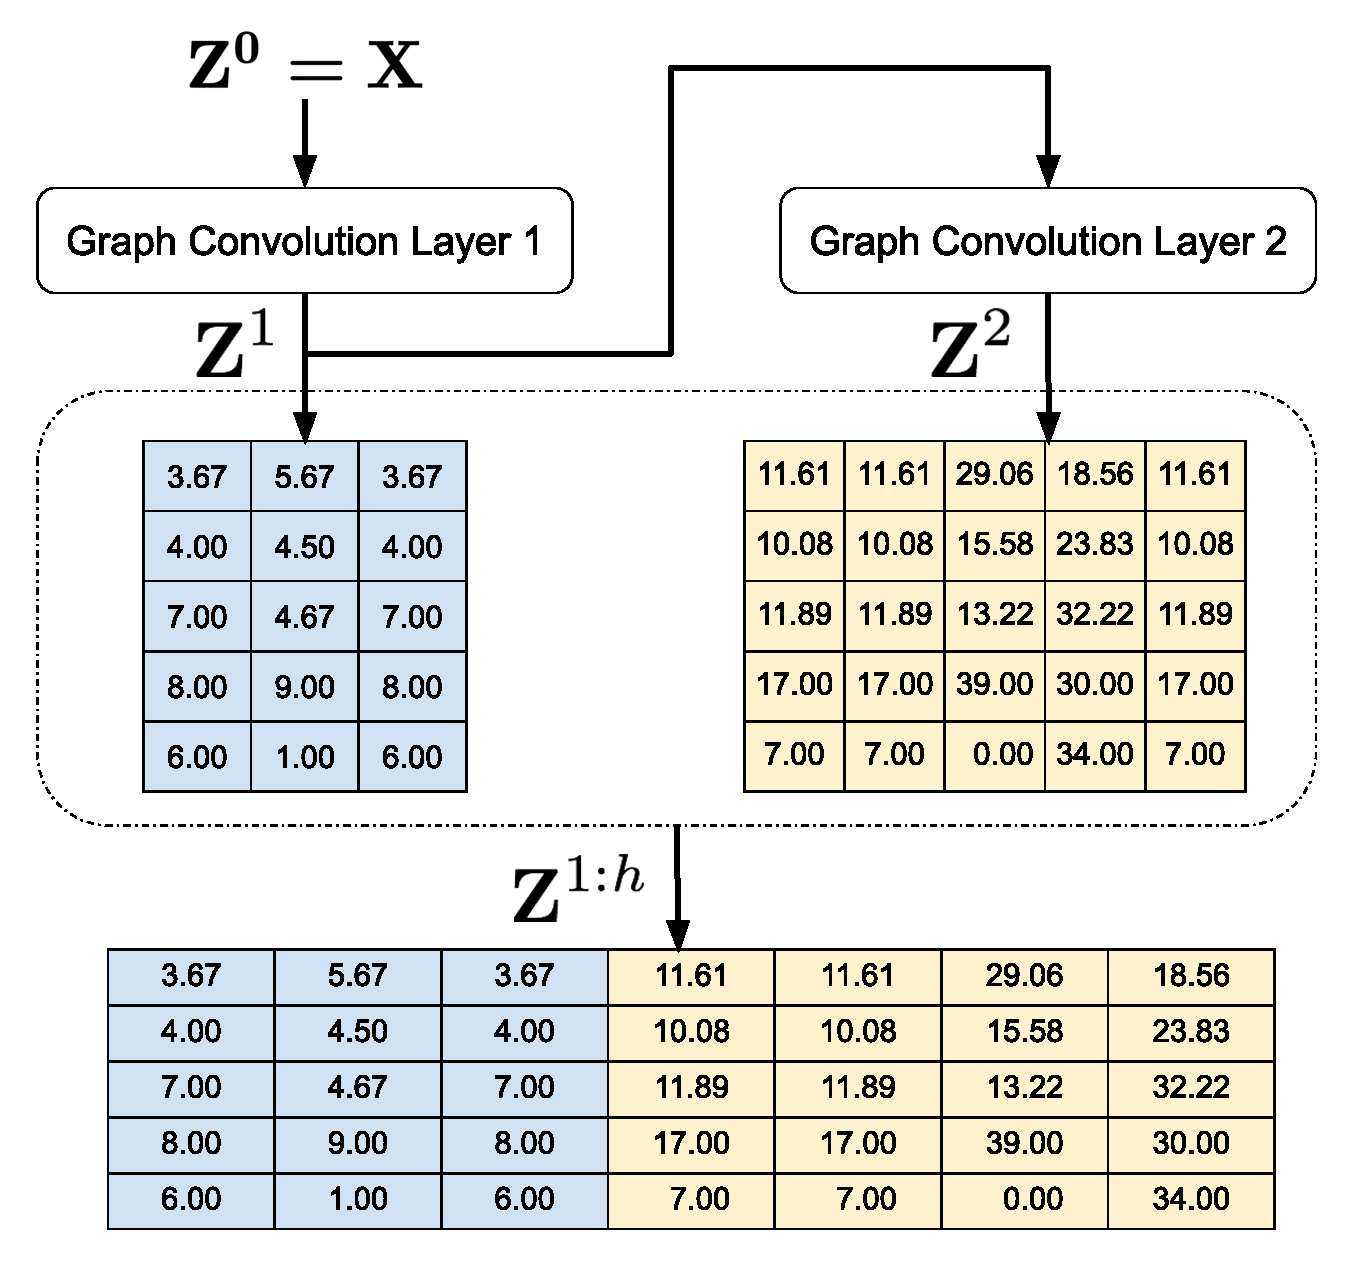
\includegraphics[width=0.90\textwidth]{Magic/figures/ExampleGraphConvolution.eps}}
\caption{Applying $h=2$ Graph Convolution Layers to Example Graph $g$}
\label{MG:Fig:ExampleGraphConvolution}
\end{figure*}

\textbf{SortPooling Layer.} Intuitively $\mathbf{Z}^{1:h}$ has $n$ rows and $\sum_{1}^{h}c_t$ column, which
corresponds to the \textit{feature descriptor} of each vertex at different scales.
The second stage, namely the \textit{sortpooling} layer,
leverages the feature descriptors to sort the vertices.
Vertices in different graphs will be put in similar positions as long as they have similar weighted feature descriptors.
The sortpooling layer starts with the last layer because $\mathbf{Z}^{h}$ is approximately
equivalent to the most refined continuous colors as in the Weisfeiler-Lehman graph kernels~\cite{WlGraphKernel}.
More specifically, vertices are first sorted by the last channel of the last layer in a decreasing order.
%When a tie on the last channel occurs, sorting will use the second last channel.
If there are $c_h$ ties on the last layer's output $\mathbf{Z}^{h}$,
sorting continues by using the second last layer's output $\mathbf{Z}^{h - 1}$, and the procedure repeats until all ties are broken.
The sortpooling layer further truncates or pads the sorted tensors by the first dimension so that it outputs $\mathbf{Z}^{sp}$ of size $k$ by $\sum_{1}^{h}c_t$.
Hence, the sortpooling process unifies the size of feature descriptors for all graphs.
Following our sample graph $g$, we visualize this process in Figure~\ref{MG:Fig:ExampleSortpool}.
Given the graph convolution result $\mathbf{Z}^{1:h}$ for the sample graph $g$ in Figure~\ref{MG:Fig:ExampleGraphConvolution},
the sortpooling layer with $k = 3$ sorts the feature descriptors (based on only the last feature channel in this example) and then truncates the two `smallest' rows.
The row of $\mathbf{Z}^{h}$ is first sorted using only the value in the last column.
The last two rows (i.e., yellow and red) are discarded from the sorted matrix as $n - k = 2 > 0$.

\textbf{Remaining Layer(s).} In the last stage, the authors of the original DGCNN\cite{Dgcnn} append a one-dimension convolution (Conv1D) layer of kernel size $\sum_{1}^{h}c_t$ and stride size $\sum_{1}^{h}c_t$.
If $F$ is the number of filters in the last one-dimension convolution layer, the sort pooling output $\mathbf{Z}^{sp}$ will be reduced to a one-dimension vector of size $k \times F$, which is then fed into a fully connected one-layer perceptron for graph classification.

\begin{figure*}[htbp]
\centerline{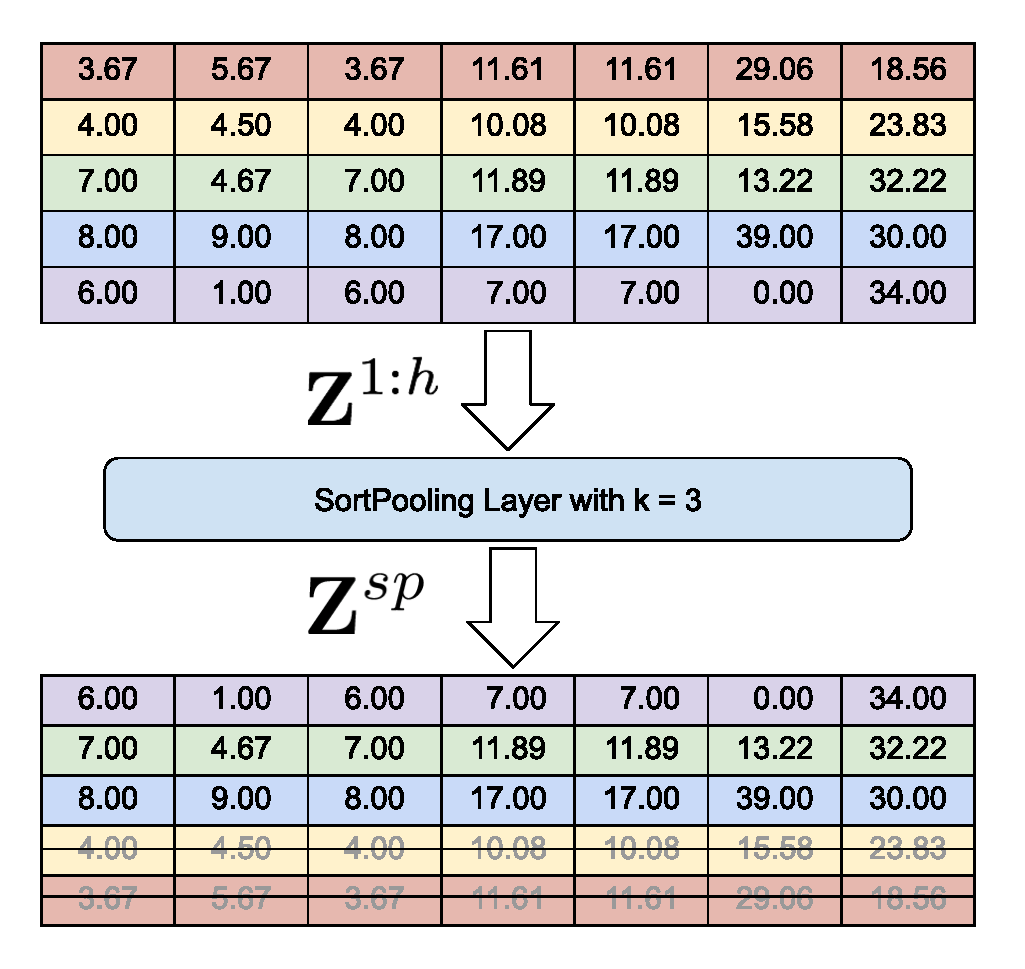
\includegraphics[width=0.90\textwidth]{Magic/figures/ExampleSortpool.eps}}
\caption{Applying Sortpooling Layer to Example Graph $g$}
\label{MG:Fig:ExampleSortpool}
\end{figure*}

\subsection{WeightedVertices Layer}
In the first extension to DGCNN, we observe that the Conv1D layer following the sortpooling layer can alternatively be of kernel size $k$, stride size $k$, and single channel.
Mathematically, a single channel Conv1D layer can be represented as a row of parameters $W \in \mathbb{R}^{1 \times k}$.
Its output $E \in \mathbb{R}^{1 \times \sum_{1}^{h}c_t}$, when fed with \textit{transposed} $\mathbf{Z}^{sp}$, will be equivalent to
\begin{equation}
    E = f(\mathbf{W} \times \mathbf{Z}^{sp})
\label{MG:Equ:WeightedVertices}
\end{equation}
%which is obviously after we notice that
This is because
\begin{equation}
    E_c = f(\sum_{i}^{k} W_i \times \mathbf{Z}^{sp}_{i, c})
\end{equation}
where $1\leq c \leq \sum_{1}^{h}c_t$, and $f$ is an element-wise nonlinear activation function.
Inspired by the graph embedding idea in\cite{GraphEmbedding}, our Conv1D layer treats each row of the sort pooling result $\mathbf{Z}^{sp}_{i}$ as the embedding of the vertices kept by the sortpooling layer.

Equivalently, Equation~(\ref{MG:Equ:WeightedVertices}) computes $E$, the embedding of the graph obtained through a weighted summation of vertex embeddings \cite{GraphEmbedding}.
For our sample graph $g$, its ``embedding" is computed in Figure~\ref{MG:Fig:ExampleWeightedVertice}, where we assume weight vector $\mathbf{W}=[0.4, 0.1, 0.5]$.
WeightVertices layer aggregates sample graph $g$'s vertex embeddings,
e.g. the output of sort pooling layer $\mathbf{Z}^{sp}$ in Figure~\ref{MG:Fig:ExampleSortpool}, to graph embedding $E$.
We choose again RELU as the nonlinear activition function $f$ for simplicity.
In reality, $\mathbf{W}$ is updated by gradient descent during the process of minimizing the classification loss.
For ease of presentation, in the remainder of the paper we refer to this special Conv1D layer after the sortpooling layer as the \textit{WeightedVertices} layer.
We replace the original Conv1D layer with the WeightVertices layer, because the WeightVertices layer leverages the graph embedding idea to make the output from the sorting pooling layer compatible with the malware classifier.

\begin{figure*}[htbp]
\centerline{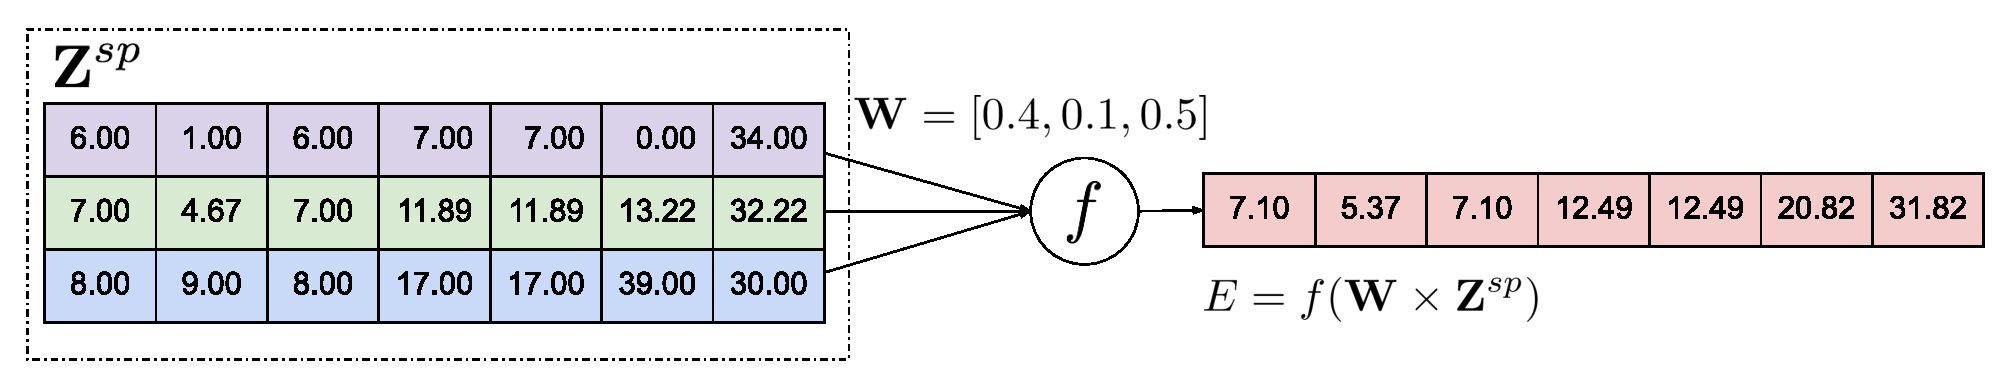
\includegraphics[width=0.90\textwidth]{Magic/figures/ExampleWeightedVertice.eps}}
\caption{Applying WeightVertices Layer to Example Graph $g$.}
\label{MG:Fig:ExampleWeightedVertice}
\end{figure*}

\subsection{AdaptiveMaxPooling: An Alternative to Sortpooling}
The intuition behind sorting from the deeper layer is to treat its output as more refined WL colors\cite{WlAlgorithm, WlGraphKernel}.
The inner sorting inside the channels of a fixed layer output is, however, less reasonable.
Besides, the Conv1D addendum is only aggregating the feature descriptors of per vertex and per convolution channel separately.

Our second extension is to apply the adaptive max pooling (AMP) on the concatenated graph convolution layer output $\mathbf{Z}^{1:h}$.
Given an set of two-dimension inputs of various sizes $\{x_i | x_i \in \mathbb{R}^{h_i \times w_i}\}$,
The AMP layer divides each input $x_i$ into a $H \times W$ grid with a sub-window size approximately to $h_i / H$ and $w_i / W$,
and then automatically chooses kernel sizes as well as convolution strides for different $x_i$.
Inside each sub-window and each channel, only the maximum element is kept in order to form the set of identical-dimension outputs $\{y_i | y_i \in \mathbb{R}^{ H \times W}\}$.
The way in which AMP works for our sample graph $g$ is illustrated in Figure~\ref{MG:Fig:ExampleAmp}.
The left top matrix $\mathbf{Z}^{1:h}_g$ represents the graph convolution output of the sample graph $g$ in Figure~\ref{MG:Fig:ExampleGraph}.
The left bottom matrix $\mathbf{Z}^{1:h}_{g'}$ represents the graph convolution output of another imaginary graph $g'$ with four vertices.
For $\mathbf{Z}^{1:h}_g$ of size $5\times 7$, adaptive max pooling's kernel size = $3 \times 3$ (shown as red shadow).
For $\mathbf{Z}^{1:h}_{g'}$ of size $4\times 7$, adaptive max pooling's kernel size = $2 \times 3$ (shown as red shadow).
For both inputs, padding = 0, stride = $2 \times 1$.
Since the dimension of the graph convolution output $\mathbf{Z}^{1:h}_g$ for $g$ is $5 \times 7$, AMP uses a max pooling kernel of size $3 \times 3$.
To show how AMP works for inputs of different dimension sizes, in Figure~\ref{MG:Fig:ExampleAmp} we also feed $\mathbf{Z}^{1:h}_{g'}$,
the graph convolution output for another graph $g'$ (not shown here), to the $3 \times 3$ AMP layer.
In this case, the kernel size is adaptively adjusted to $2 \times 3$.

We have two motivations for using AMP at the end of the graph convolution layer.
In addition to unifying the convolution layer output $\mathbf{Z}^{1:h}$, AMP empowers us to aggregate $\mathbf{Z}^{1:h}$
across the dimensions of both feature channels and graph vertices simultaneously,
which enables us to capture informative features that vary only by location.
This is easily accomplished by applying a two-dimension convolution (Conv2D) layer with an arbitrary number of filters before the AMP layer.
The output of the AMP layer is further fed into a multiple-Conv2D-layer neural network, inspired by VGG~\cite{VGG}, to predict the probability distribution of the malware families that the input CFG should belong to.

\begin{figure*}[htbp]
\centerline{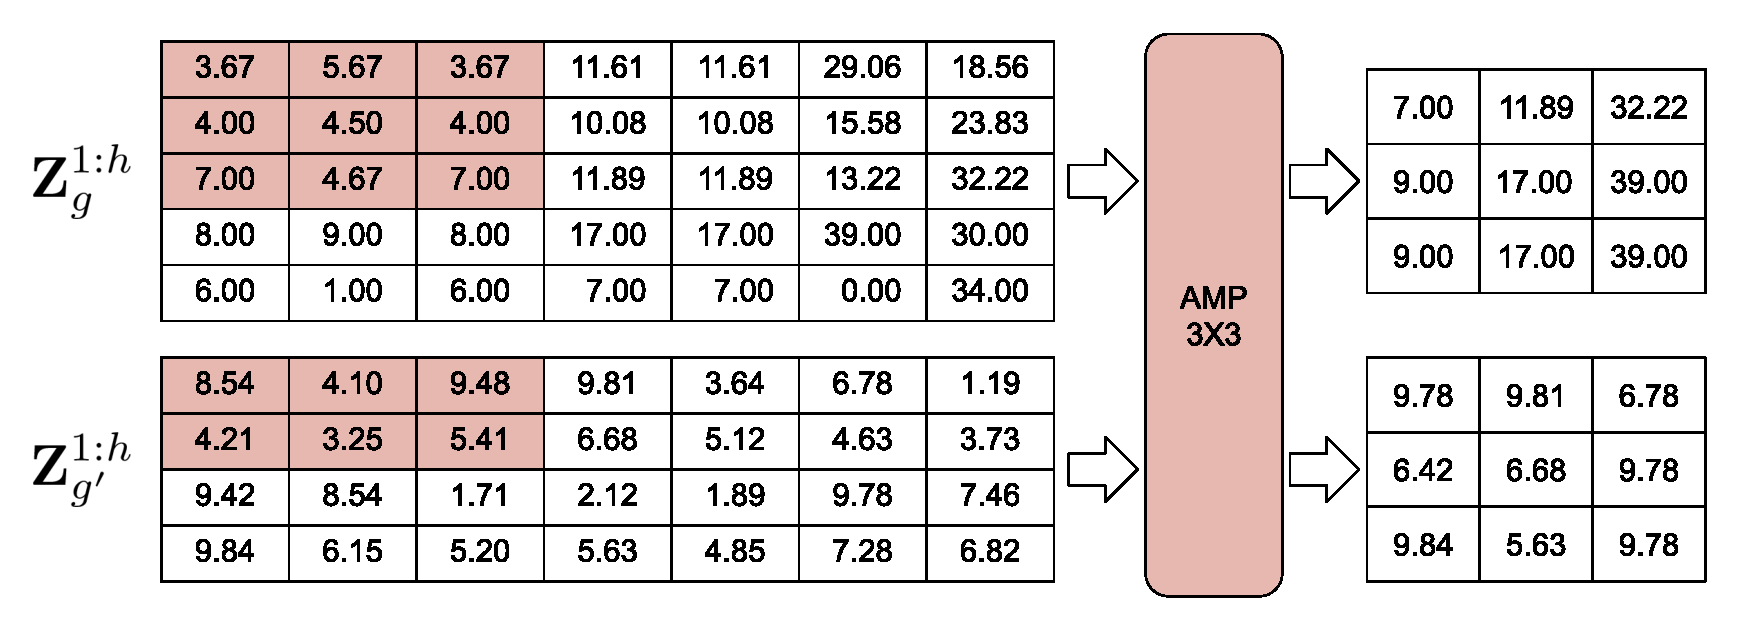
\includegraphics[width=0.90\textwidth]{Magic/figures/ExampleAmp.eps}}
\caption{Applying AdaptiveMaxPooling Layers to Example Graph $g$.}
\label{MG:Fig:ExampleAmp}
\end{figure*}

\Section{Implementation}
\label{VT:Sec:Implementation}

The implementation of the virtual time system and its integration with Mininet-Hifi (the latest version of Mininet) is composed of three parts,
as shown in Figure~\ref{VT:Fig:VTMininetHifi}.
First, we built a lightweight and independent middleware in the Linux kernel to provide virtual time support to user-space software.
Second, we slightly modified the initialization procedure of Mininet with two additional python modules to realize (adaptive) virtual time in Mininet.
Third, we discuss our design to enable transparent support of virtual time for applications running in the containers.

\begin{figure}
    \centering
    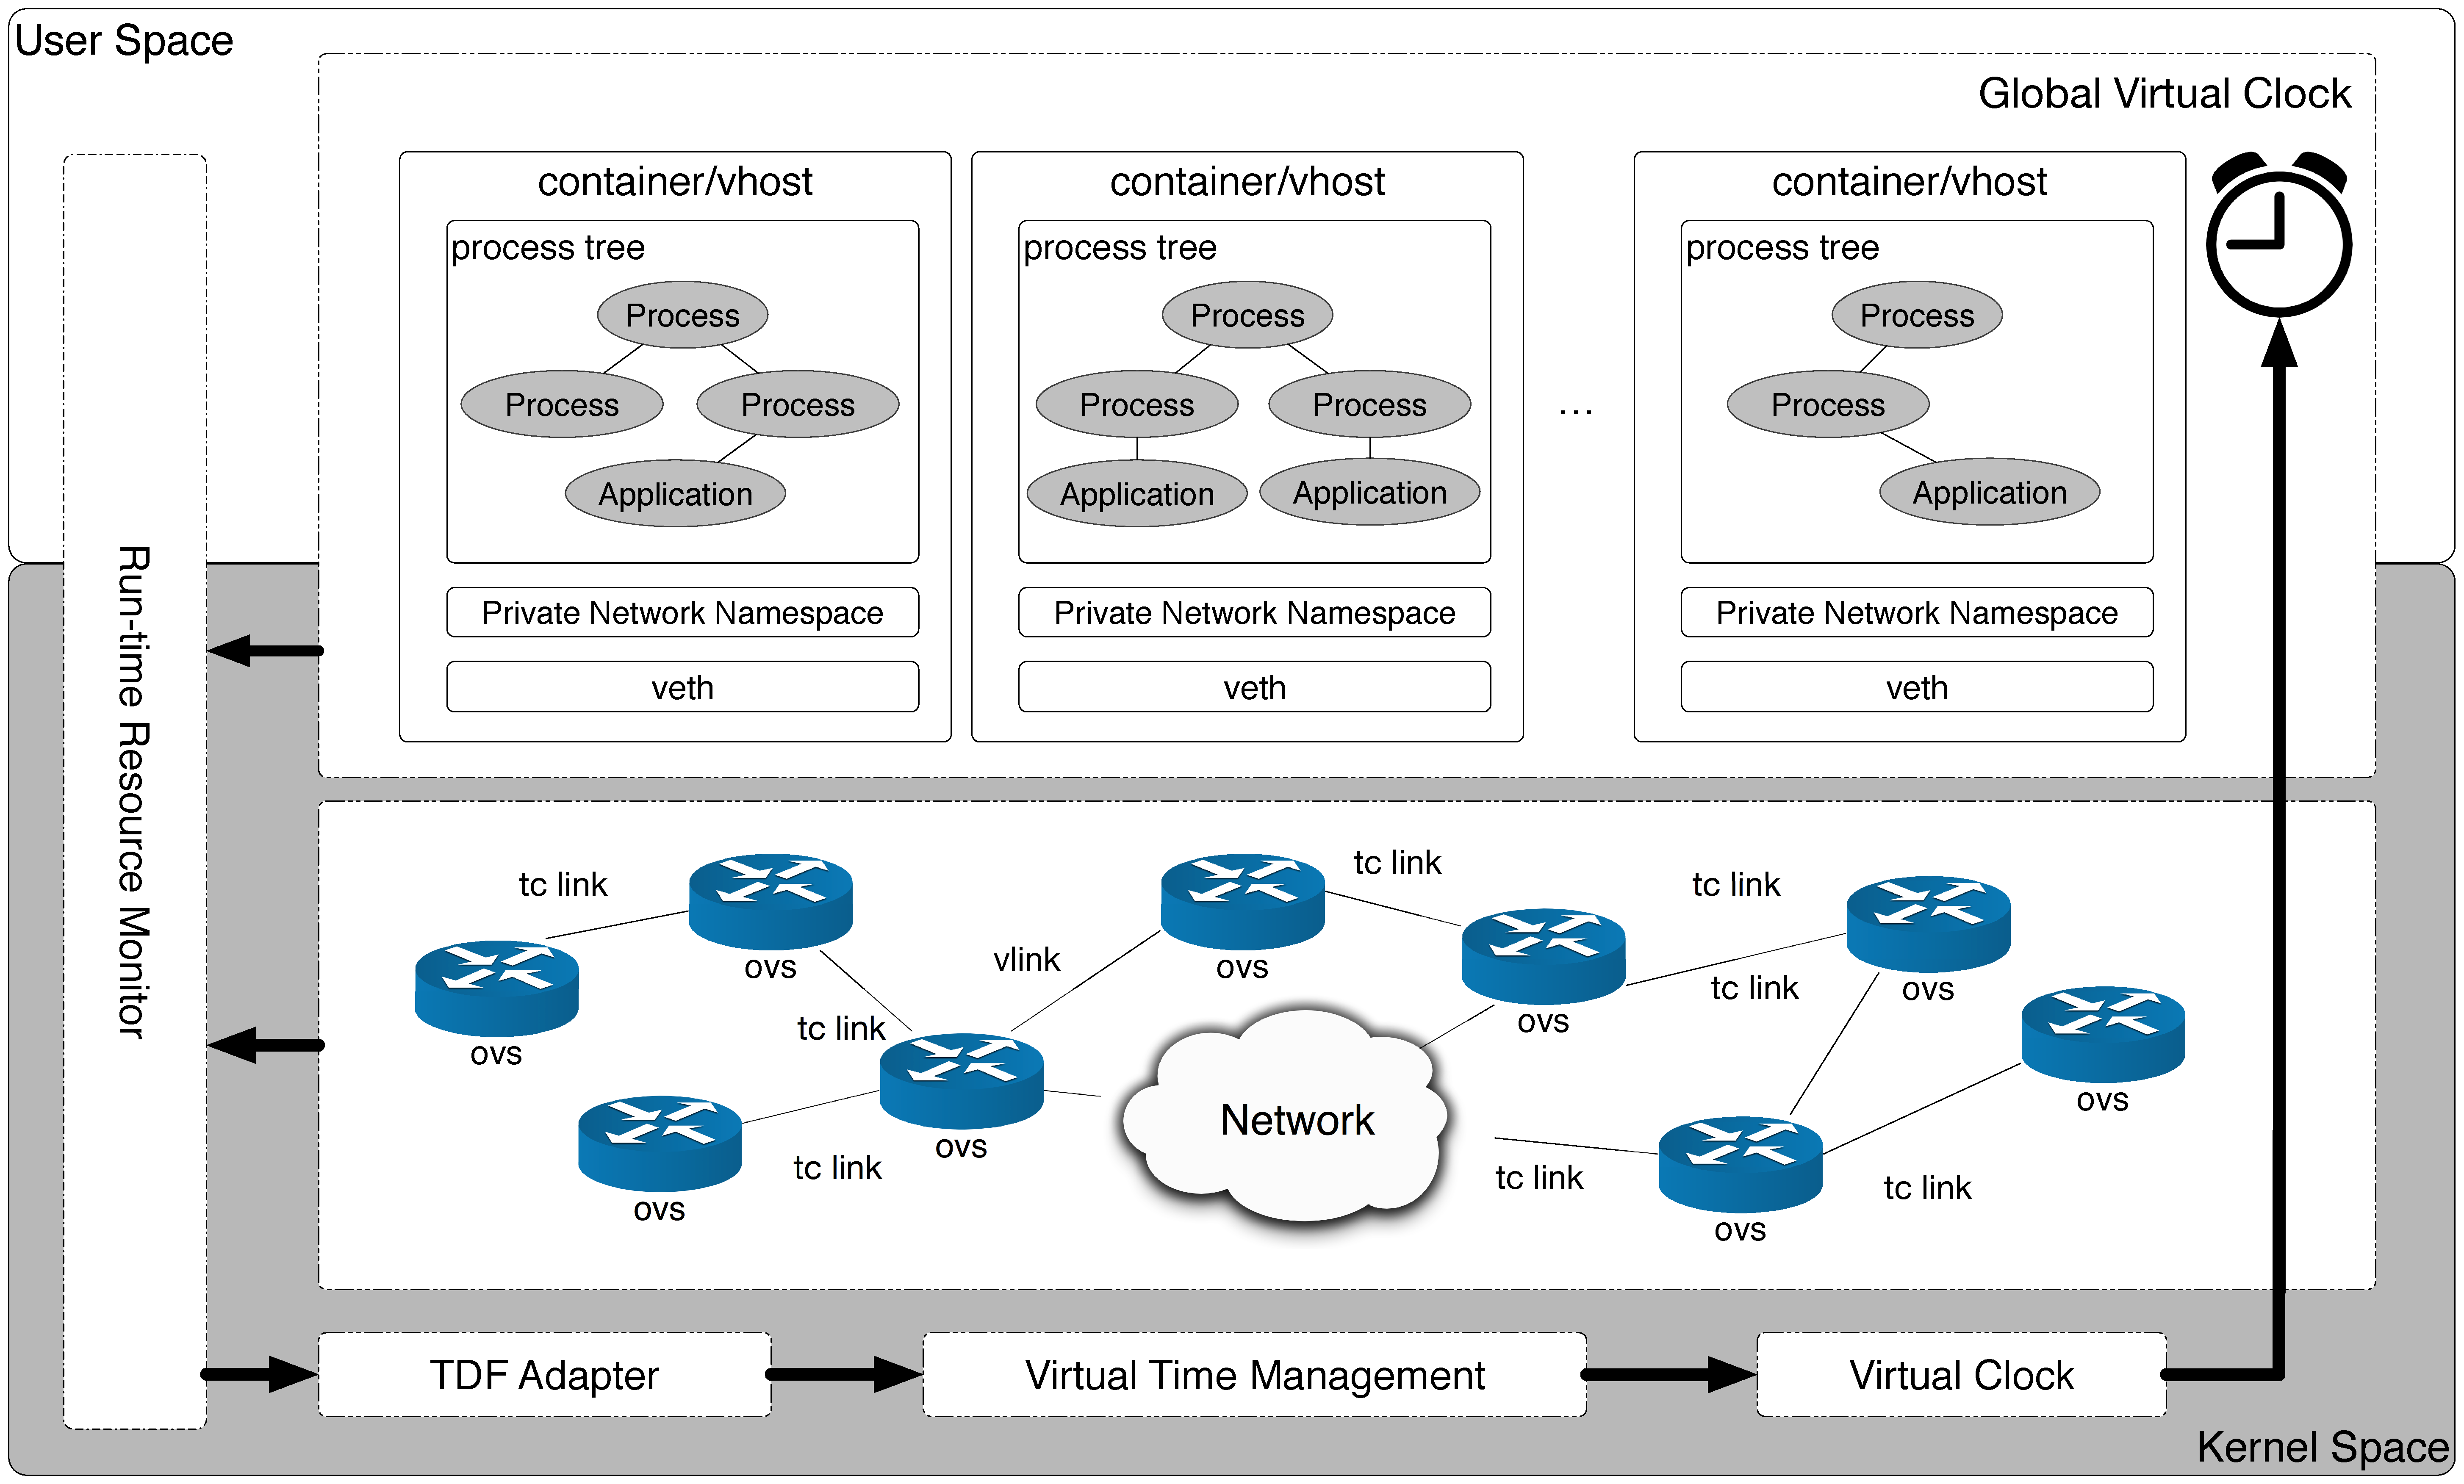
\epsfig{file=VirtualTime/figures/VT-Mininet-Hifi.eps, width=0.9\textwidth}
    \caption{Integration of Mininet-Hifi and Virtual Time}
    \label{VT:Fig:VTMininetHifi}
\end{figure}

\Subsection{Modification in Linux Kernel}
\paragraphbe{Timing-related Kernel Modifications.}
\label{VT:SubSec:ExtendLinuxKernel}
Our implementation is based on a recent Linux kernel 3.16.3 with no third-part library dependency.
To make a process have its own perception of time, we added the following four new fields in the \texttt{task\_struct} struct type.
\begin{itemize}
    \item \texttt{physical\_start\_ns} represents the starting time that a process detaches from the system clock and begins to use the virtual time, in nanoseconds.
    \item \texttt{physical\_past\_nsec} represents how much physical time has elapsed since the last time the process requested the current time, in nanoseconds
    \item \texttt{virtual\_start\_nsec} represents the starting time that a process detaches from the system clock and uses the virtual time, in nanoseconds 
    \item \texttt{virtual\_past\_nsec} represents how much virtual time has elapsed since the last time the process requested the current time, in nanoseconds
    \item \texttt{freeze\_start\_ns} represents the starting time that a process or a process group is frozen. It is always zero for a non-frozen process.
    \item \texttt{freeze\_past\_ns} represents the cumulative time, in nanoseconds, that a running process or a process group remains in the frozen state.
    \item \texttt{dilation} represents the TDF of a time-dilated process
\end{itemize}

\begin{algorithm}[ht]
    \DontPrintSemicolon
    \KwIn{$tk = $ C struct \texttt{task\_struct} representing a process in Linux kernel \newline
    $dilation = $ value of time dilation factor}
    \SetKwProg{Fn}{Function}{}{\KwRet}
    \SetKwFunction{InitVT}{init\_virtual\_time}
    \SetKwFunction{GetNS}{getnstimeofday}
    \SetKwFunction{TSNS}{timespec\_to\_ns}
    \Fn{\InitVT{$tk$, $dilation$}} {
        \If {$dilation > 0$} {
            $tk.virtual\_start\_nsec \gets 0$ \;
            $ts \gets$ \GetNS{} \;
            $tk.virtual\_start\_nsec \gets$ \TSNS{$ts$} \;
            $tk.virtual\_past\_nsec \gets 0$ \;
            $tk.physical\_past\_nsec \gets 0$ \;
            $tk.dilation \gets dilation$
        }
    }
    \caption{Initialize Virtual Time}
    \label{VT:Alg:InitVirtualTime}
\end{algorithm}

\begin{algorithm}[ht]
    \DontPrintSemicolon
    \KwIn {$p = $ the current running process in Linux kernel \newline
    $ts = $ current wall clock time \newline
    $tdf = p.dilation$}
    \SetKwProg{Fn}{Function}{}{\KwRet}
    \SetKwFunction{UpdatePPN}{update\_physical\_past\_nsec}
    \SetKwFunction{UpdateVPN}{update\_virtual\_past\_nsec}
    \SetKwFunction{DoDilate}{do\_virtual\_timekeeping}
    \SetKwFunction{TSNS}{timespec\_to\_ns}
    \SetKwFunction{NSTS}{ns\_to\_timespec}
    \Fn{\UpdatePPN{$ts$}} {
        $now \gets \TSNS{$ts$}$ \;
        $delta\_ppn \gets now - p.physical\_past\_nsec - p.physical\_start\_nsec - p.freeze\_past\_nsec$ \;
        $p.physical\_past\_nsec += delta\_ppn$ \;
        \KwRet{$delta\_ppn$} \;
    }
    \Fn{\UpdateVPN{$delta\_ppn$}} {
        $delta\_vpn \gets 0$ \;
        \If {$tdf > 0$} {
            $delta\_vpn \gets delta\_ppn / tdf$ \;
            $p.virtual\_past\_nsec += delta\_vpn$ \;
        }
        \KwRet{$delta\_vpn$}
    }
    \Fn{\DoDilate{$ts$}} {
        \If {$p.virtual\_start\_ns > 0$} {
            $delta\_ppn \gets \UpdatePPN{ts}$ \;
            $delta\_vpn \gets \UpdateVPN{delta\_ppn, tdf}$ \;
            $virtual\_now = p.virtual\_start\_nsec + p.virtual\_past\_nsec$ \;
            $virtual\_ts = \NSTS{virtual\_now}$ \; 
            $ts.tv\_sec = virtual\_ts.tv\_sec$ \;
            $ts.tv\_nsec = virtual\_ts.tv\_nsec$ \;
        }
    }
    \caption{Virtual Timekeeping Algorithm}
    \label{VT:Alg:VirtualTimeKeeping}
\end{algorithm}

\begin{algorithm}
    \DontPrintSemicolon
    \KwIn {$tsk = $ the process/container in Linux kernel to be frozen or unfrozen}
    \SetKwProg{Fn}{Function}{}{\KwRet}
    \SetKwFunction{Freeze}{freeze}
    \SetKwFunction{Unfreeze}{unfreeze}
    \SetKwFunction{PopulateFreeze}{populate\_frozen\_time}
    \SetKwFunction{KillGroup}{kill\_pgrp}
    \SetKwFunction{TaskGroup}{task\_pgrp}
    \SetKwFunction{GetNS}{getnstimeofday}
    \SetKwFunction{TSNS}{timespec\_to\_ns}
    \Fn{\Freeze{tsk}} {
        \KillGroup{\TaskGroup{tsk}, \texttt{SIGSTOP}, 1} \;
        $ts = $\GetNS{} \;
        $tsk.freeze\_start\_nsec \gets$ \TSNS{ts} \;
    }
    \Fn{\PopulateFreeze{tsk}} {
        \ForEach {child $\in$ tsk.children} {
            $child.freeze\_past\_nsec \gets tsk.freeze\_past\_nsec$ \;
            \PopulateFreeze{child} \;
        }
    }
    \Fn{\Unfreeze{$tsk$}} {
        $ts = $\GetNS{} \;        
        $now \gets$ \TSNS{ts} \;
        $tsk.freeze\_past\_nsec += now - tsk.freeze\_start\_nsec$ \;
        $tsk.freeze\_start\_nsec \gets 0$ \;
        \PopulateFreeze{tsk} \;
        \KillGroup{\TaskGroup{$tsk$}, \texttt{SIGCONT}, 1} \;
    }
    \caption{Freeze and Unfreeze Linux Container}
    \label{VT:Alg:Freeze}
\end{algorithm}


Algorithm~\ref{VT:Alg:InitVirtualTime} and~\ref{VT:Alg:VirtualTimeKeeping} give the details about how we implement the time dilation. 
To preserve an accurate virtual clock in the kernel, we added a private function \texttt{do\_virtual\_timekeeping}
in the Linux's timekeeping subsystem to keep tracking the dilated virtual time based on the physical time passed and TDF. 
Based on process's \texttt{virtual\_start\_nsec}, the system determines the type of time to return, i.e., the physical system clock time or the virtual time.

\texttt{virtual\_start\_nsec} in \texttt{init\_virtual\_time} should first be initialized to zero so that the next \texttt{gettimeofday}
always returns the undilated time to compute and record the exact physical time that a process starts to use virtual time.
To return the accurate virtual time upon requests, the duration since the last call to \texttt{do\_virtual\_timekeeping} is calculated and precisely scaled with TDF. 
To enable virtual time support for a wide range of timing-related system calls,
we extensively traced the routines in Linux's subsystems that request timing information (such as \texttt{getnstimeofday},
\texttt{ktime\_get}, \texttt{ktime\_get\_ts}, etc.), and modified them to properly invoke \texttt{do\_virtual\_timekeeping}.

The algorithm to freeze/unfreeze processes is shown in Algorithm~\ref{VT:Alg:Freeze},
and is implemented in the Linux kernel.
After stopping a group of processes, we record the  current time for calculating the process frozen duration once we unfreeze the process.
Note that sending \texttt{SIGCONT} to all processes is behind the time keeping function.
The reason is that if we resume the process group first, an unfrozen process may be scheduled to run,
and possibly query time before we complete populating the \texttt{freeze\_past\_ns} within the entire container.
We also develop a user space utility program \texttt{freeze\_all\_proc}.
This program can freeze and unfreeze multiple hosts in parallel.
In particular, it spawns one \texttt{pthread} for every network host to write its freeze entry in the Proc system.
Since the network emulator always pauses or resumes all hosts, this optimization significantly reduces the running overhead in large-scale network settings.

The virtual file system provides an interface between the kernel and the user space.
Since virtual time is a per-process property, it is more efficient to create a \texttt{/proc}
file entry for the associated processes rather than adding system calls.
The virtual time interface consists of two extra file entries under \texttt{/proc/\$pid}.
\begin{itemize}
    \item \texttt{/proc/\$pid/dilation} A process \texttt{\$pid} can enable and disable virtual time, as well as change a new time dilation factor (TDF).
        To support fractional dilation values, a TDF of $x$ is stored in this entry as $1000x$,  since floating point numbers are rarely supported in the Linux kernel.
    \item \texttt{/proc/\$pid/freeze} We can freeze and unfreeze a process \texttt{\$pid} according to the written boolean value.
        A value 1 freezes the entire process group and a value 0 resumes all the processes in this group.
\end{itemize}

We make a distinction between regular processes and virtual-time enabled processes. In other words, the \texttt{/proc/\$pid/freeze} entry is only valid only if \texttt{/proc/\$pid/dilation}  already has a non-zero value. The emulator can enable a container with virtual time by writing 1000 to the \texttt{dilation} proc file entry. This will turn on the freeze/unfreeze capability without unnecessarily modifying the clock speed. In this work, we use a process calling system call \texttt{unshare()} with flag \texttt{CLONE\_NEWTIME} to enable virtual time.
This design is motivated and tailored to be compatible with Mininet's programming interface.
\paragraphbe{Process-related Kernel Modifications.}
To enable the virtual time perception to processes running in a network emulator, we added the following new system calls.
\begin{itemize}
    \item \texttt{virtualtimeunshare} is essentially the \texttt{unshare} system call with time dilation inputs.
        It is used by container-based emulators, such as Mininet, to create emulated nodes.
        \texttt{virtualtimeunshare} creates a new process with a TDF in a different \texttt{namespace} of its parent process according to \texttt{flags}.
    \item \texttt{settimedilaitonfactor} offers an interface to change the TDF of a process.
        Note that a command executed in an emulated host is equivalent to forking a shell command executed by \texttt{bash}. 
        Therefore, adjusting a process' TDF requires the change of the calling process' parent (e.g., host's \texttt{bash}),
        which occasionally would lead to tracing back to the root of the process tree, especially in the case of dynamic TDF adjustment. 
\end{itemize}

We also modified the \texttt{do\_fork} system call to initialize the virtual-time-related attributes of a process,
such as using the variable \texttt{stack\_size} to pass the TDF value. 
Another option is to set TDF to a default value in \texttt{virtualtimeunshare} and
then relies on explicitly invoking \texttt{settimedilationfactor} to set desired TDF;
this method prevents modifying the interface of creating \texttt{namespace} in traditional Linux. 
Functions in \texttt{timekeeping.c} were modified to invoke \texttt{do\_dilatetimeofday}
in order to return the virtual time to system calls like \texttt{gettimeofday} and other kernel routines that request timing information.


\paragraphbe{Networking-related Kernel Modifications.}
In this work, we focus on capturing all the related system calls and kernel routings to support virtual time in Linux container with the application of Mininet. 
One particular case related to Mininet is the usage of \texttt{tc}, a network quality-of-service control module in Linux~\cite{TrafficControl}. 
For instance, we can use \texttt{tc} to rate-limit a link to 100 Mbps using Hierarchic Token Bucket (HTB) \texttt{qdisc} in Mininet. If the TDF is set to 8, the link bandwidth would be approximately 800 Mbps from the emulated hosts' viewpoints as we observed from the time-dilated \texttt{iperf3} application.

As a network module in Linux, \texttt{tc} does not reference Linux kernel's time as the way user application does. 
Therefore, \texttt{tc} is transparent to our virtual time system. One way to solve this problem is to modify the network scheduling code in kernel to provide \texttt{tc} with a dilated traffic rate. 
In the earlier example with TDF set to 8, the experiment will run 8 times slower than the real time, and we can configure \texttt{tc}'s rate limit as $rate/TDF=12.5$ Mbps to emulate a 100 Mbps link. 
Note that we only tailored HTB in \texttt{tc}, which is the default \texttt{qdisc} used by Mininet. 
We will generalize the mechanism to other \texttt{qdiscs} including HFSC (Hierarchical Fair Service Curve) and TBF (Token Bucket Filter) in the future.

\Subsection{Modification in Network Emulator}
\paragraphbe{Virtual-Time-Enabled Mininet.}
\label{VT:SubSec:ImplementMininet}
%Mininet uses Linux's container \cite{LXC} to enable scalable network emulation. 
Containers allow groups of process running on the same kernel to have independent views of system resources, such as process IDs, file systems and network interfaces. 
We add the virtual time property to a container's \texttt{namespace}~\cite{LinuxNamespace} so that every container can have its own virtual clock. 
We design our system in the way that minimal modifications of Mininet are needed for integration, so that the virtual time system can be easily extended to other Linux-container-based applications. 

We modified the initialization procedure of Mininet, in particular, the \texttt{mnexec} program in Mininet, to process two additional parameters. 
When we create \texttt{Node}s in Mininet (hosts, switches, and controllers are all inherited from \texttt{Node}), users can feed in a TDF argument with \texttt{virtualtimeunshare} (as a replacement of \texttt{unshare}) with \texttt{-n} option. 
This way, a system-wide TDF can be conveniently set for all the emulated hosts. We also provide the ability to dynamically adjust the TDF for every emulated host during runtime. 
To do that, we added a new option \texttt{-t} in \texttt{mnexec} to invoke the aforementioned system call \texttt{settimedilaitonfactor} to do the actual TDF adjustment. 
The two modifications enable the integration of virtual time in Mininet, and also serve as the basis of the adaptive TDF management.

\paragraphbe{Adaptive TDF Scheduling.}
To optimize the performance of the virtual-time-enabled Mininet, we developed an adaptive TDF scheduler
through two python modules \texttt{MininetMonitor} and \texttt{DilationAdaptor}
(refer to Emulation Monitor and Time Dilation Adaptor in Figure~\ref{VT:Fig:ContainerVirtualTime})
to accelerate the experiment speed while preserving high fidelity.

\texttt{MininetMonitor} is responsible to monitor the CPU usage of the entire emulation system,
consisting of a group of processes including the Mininet emulator, the Open vSwitch module, and emulated nodes (e.g., SDN controllers, hosts and switches). 
Also, applications are dynamically created, executed and destroyed within containers, in the form of child processes of their parent containers. 
\texttt{MininetMonitor} utilizes the \texttt{ps} command to collect the group's aggregate CPU percentage
and periodically computes and passes the average CPU load statistics to \texttt{DilationAdaptor}. 
The core of \texttt{DilationAdaptor} is an adaptive algorithm to calculate an appropriate \textit{TDF}.
%Only after receiving a new \textit{TDF} can Mininet pause the experiment and update its global time dilation factor. Otherwise it enters the next Epoch directly. 
Global \textit{TDF} updating was achieved by invoking the \texttt{mnexec\ -t\ tdf} program for every running host. 


% Algorithm \ref{Alg-AdaptiveTDF} illustrates our adaptive TDF scheduling, and we implemented it as a threshold-based \texttt{DilationAdaptor}. 
% %From the input fed by \texttt{MininetMonitor}, \texttt{DilationAdaptor} first define current load status. The key idea here is: if emulator is overloaded, we increase TDF with a large value; if it is underloaded, we may consider decrease TDF with a large value. 

% \algnewcommand\algorithmicswitch{\textbf{switch}}
% \algnewcommand\algorithmiccase{\textbf{case}}
% \algnewcommand\algorithmicassert{\texttt{assert}}
% \algnewcommand\Assert[1]{\State \algorithmicassert(#1)}%
% % New "environments"
% \algdef{SE}[SWITCH]{Switch}{EndSwitch}[1]{\algorithmicswitch\ #1\ \algorithmicdo}{\algorithmicend\ \algorithmicswitch}%
% \algdef{SE}[CASE]{Case}{EndCase}[1]{\algorithmiccase\ #1}{\algorithmicend\ \algorithmiccase}%
% \algtext*{EndSwitch}%
% \algtext*{EndCase}%

% \algrenewcommand{\algorithmiccomment}[1]{\hskip1em$/*$ #1 $*/$}
% \begin{algorithm}
% \caption{Adaptive Time Dilation Factor Scheduling}\label{Alg-AdaptiveTDF}
% \begin{algorithmic}[1]
% \State{Decide emulation $state$ through the resource indicator}\Comment{e.g., CPU utilization}
% \State{$MAX$ denotes the maximum allowed TDF value.}
% \State{$\Delta_{large}, \Delta_{small}$ denote the customizable large and small adjustment}
% \Switch{$state$}
% 	\Case{$OVERLOADED$}
% 		\State{$TDF_{new}=TDF_{prev}+\Delta_{large}$}
% 	\EndCase
% 	\Case{$WARNING$}
% 		\State{$TDF_{new}=TDF_{prev}+\Delta_{small}*2$}
% 	\EndCase
% 	\Case{$MODERATE$}
% 		\If{$TDF_{prev} == MAX$}
% 			\State{$TDF_{new}=TDF_{prev}-\Delta_{large}$}
% 		\ElsIf{$TDF_{prev} > \Delta_{small}$}
% 			\State{$TDF_{new}=TDF_{prev}-\Delta_{small}$}
% 		\Else
% 			\State{$TDF_{new}=TDF_{prev}$}%\Comment{Do not change TDF}
% 		\EndIf
% 	\EndCase
% 	\Case{$LIGHT$}
% 		\If{$TDF_{prev} > \Delta_{large}*2$}
% 			\State{$TDF_{new}=TDF_{prev}-\Delta_{large}$}
% 		\Else
% 			\State{$TDF_{new}=TDF_{prev}-\Delta_{small}*2$}
% 		\EndIf
% 	\EndCase
% \EndSwitch
% %\State{return $TDF_{new}$}
% \end{algorithmic}
% \end{algorithm}

Our adaptive virtual time scheduling design is similar to the one used in~\cite{NtwkEmultAdaptVirtTime} in spirit with two major differences. 
First, both techniques target on different platforms. 
Our technique is applied to Linux-container-based network emulation to support scalable SDN experiments,
and theirs uses virtual routing and executes OpenVZ instances inside Xen. 
Second, their solution needs be deployed on a cluster to emulate a medium-scale network, which results in much higher communication overhead in two types:
(1) every VM's monitor needs to report the CPU usage, and
(2) the adaptor needs to send new TDF to every VM. 
Therefore, the message transmission delay in LAN and the processing delay in protocol stacks contributes to the overall communication delay. 
In contrast, \texttt{MininetMonitor} runs as a lightweight background thread in Mininet,
and \texttt{DilationAdaptor} is simply a python object that Mininet has a reference to. 
The communication in our system is through synchronized queues and method invocations, which is much faster. 

\Subsection{Virtual Time Support for Network Applications}
\label{VT:SubSec:ModificationApplications}
Network applications running inside containers (e.g., \texttt{iperf3}~\cite{iperf3} or \texttt{ping}) should also use virtual time. 
We do not need to modify the application code because they are running as child processes of Mininet's hosts. 
A child process always copies its parent's \texttt{task\_struct} when it is forked including the same \texttt{dilation} and \texttt{virtual\_start\_nsec} values. 
Although \texttt{virtual\_start\_nsec} does not present the virtual starting time of the child process,
our algorithm is designed to work with relative values since it does necessary initial processes during \texttt{do\_fork}. 
When applications inquire about the system time,
the modified kernel knows that they are using virtual clock and return the virtual clock time instead of the system clock time.

One issue we notice is that the 64-bit Linux kernel running on Intel-based architectures provides the Virtual Dynamic Shared Object (vDSO)
and the \texttt{vsyscall} mechanism to reduce the overhead of context switches caused by the frequently invoked system calls,
for example, \texttt{gettimeofday} and \texttt{time}~\cite{VDSO}. 
Therefore, applications may bypass our virtual-time-based system calls unless we explicitly use the \texttt{syscall} function.
Our solution is to disable vDSO with respect to \texttt{\_\_vdso\_gettimeofday} in order to transparently offer virtual time to applications in the containers.


\section{Experimental Evaluation}
\label{MG:Sec:Experiment}

We evaluate the performance of \sysname using two large malware datasets, each with more than 10,000 samples, and present our experimental results in this section.

\subsection{Malware Datasets}
The first dataset, which we refer to as the \textit{MSKCFG} dataset, includes the CFGs derived from the malware files used in the 2015 Microsoft Malware Classification Challenge hosted by Kaggle~\cite{MsAcfgDataset}. The dataset contains samples that fall into nine families: \{Ramnit, Lollipop, Kelihos\_ver3, Vundo, Simda, Tracur, Kelihos\_ver1, Obfuscator.ACY, Gatak\}.
Figure~\ref{MG:Fig:MSKCFGLabelDist} presents the number of samples in each of these nine malware families in the dataset.
%The identification of benign code is not in the scope of the contest, and all the input files are supposed to be malicious.
In the competition, Kaggle provided 10,868 labeled malware samples as the training dataset, for each of which two files were given.
% Kaggle used another 10,873 malware samples, whose labels remained unknown to participants, to rank the submissions.
% We ignored 10 `empty'\footnote{A file is \textit{empty} if it contains only character `??', which means the data provider erased these byte information for certain reasons.} .byte files in training set and 13 empty ones in testing set respectively.
%Two files were given for each malware is represented as two files in the dataset.
The first file contains the raw binary content in a hexadecimal representation (referred as .byte file in the following discussion).
The second file is the corresponding assembly code of the binary code, which was generated with the IDA Pro tool~\cite{bib:idapro} (referred as .asm file in the following discussion).
The correctness of the .asm file is not guaranteed because PE headers were erased from the raw malware files for sterility before they were disassembled and sophisticated binary packing techniques may also prevent reverse engineering tools from disassembling the malware correctly~\cite{BinaryUnpacking}. 
In our experiments, only the .asm files were used for malware classification.
We generated a total number of 10,868 ACFGs from the training .asm files, which took approximately 17 hours to finish, or averagely 5.8 seconds per malware instance,
using a commodity desktop equipped with Intel Core i7-6850K CPU and 64 GB memory.
%These ACFGs are denoted as the \textit{MSKCFG} dataset hereafter.

Another dataset, which we refer to as \textit{YANCFG}, includes the CFGs of 16,351 binary executable files which were used in \cite{YanDataset}.
%The original dataset contains hexadecimal bytes from the original binary file and the features from both dynamic execution traces and PE headers.
%However, the dataset given to us are CFG format files.
Similar to the MSKCFG dataset, the PE headers were not available to us for malware classification from the second dataset. All the CFGs were labeled with a majority voting scheme based on the detection results of five major AV scanners returned by the VirusTotal online malware analysis service~\cite{VirusTotal}.
All the CFGs belong to 12 distinct malware families: \{Bagle, Benign, Bifrose, Hupigon, Koobface, Ldpinch, Lmir, Rbot, Sdbot, Swizzor, Vundo, Zbot, Zlob\}.
Figure~\ref{MG:Fig:YANCFGLabelDist} depicts the number of samples for each of these 12 families in the dataset.
These CFGs were further converted to their corresponding ACFGs by MAGIC within 6.8 hours using the same desktop machine as mentioned above.
%After the 6.8-hour CFG-to-ACFG conversion, we obtained 16,351 ACFGs.% further discarded 1,976 empty graphs.
%These ACFGs are stored together and referred as \textit{YANCFG} as a whole dataset.
%For clarity, we refer the second dataset as \textit{YANCFG}.
%We plan to make the resultant ACFGs on both public and private datasets available to the research community alongside with the system implementation of \sysname.


We did not merge two malware datasets in our experiments due to the following reasons.
Firstly, the YANCFG dataset carries pre-processed CFGs,
while we developed our own parser to extract CFGs from the malware assembly code in the Microsoft dataset (see Section~\ref{MG:SubSec:BuildCfg}).
% The differences in the methods used to extract CFGs from the two datasets may lead to inconsistent CFG representations for model training.
The CFG extracted from the MSKCFG dataset by our own parser has different low-level feature representation from that of the CFGs pre-given in YANCFG;
so they cannot be applied to one model.
Secondly, testing MAGIC on datasets collected from independent sources also allows us to gain insights into its generality when applied in different operational environments.

\begin{table*}[htbp]
\caption{Hyperparameters and Search Ranges during Tuning}
\begin{center}
\begin{tabular}{l|r|r|r}
\hline
Hyperparameter & Choice or Value Range & Best Model for MSKCFG & Best Model for YANCFG \\
\hline
\hline
Pooling Type & [Adaptive Pooling, Sort Pooling] & Adaptive Pooling &  Adaptive Pooling\\
\hline
Pooling Ratio & [0.2, 0.64] & 0.64 & 0.2 \\
\hline
Graph Convolution Size & [(32, 32, 32, 1)\tablefootnote{Only for sort pooling}, (32, 32, 32, 32), (128, 64, 32, 32)] & (128, 64, 32, 32) & (32, 32, 32, 32)\\
\hline
Remaining Layer\tablefootnote{Applicable only when set \textit{pooling type} to sort} & [1D Convolution Layer, WeightVertices Layer] & Not Applicable &  Not Applicable \\
\hline
2D Convolution Channels\tablefootnote{Applicable only when set \textit{pooling type} to adaptive pooling} & [16, 32]  & 16 & 16 \\
\hline
1D Convolution Channel Pairs\tablefootnote{Applicable only when set \textit{pooling type} to sort pooling and \textit{remaining layer} to 1D convolution} & [(16, 32)] & Not Applicable & Not Applicable \\
\hline
1D Convolution Kernel Size\tablefootnote{Applicable only when set \textit{pooling type} to sort pooling and \textit{remaining layer} to 1D convolution} & [5, 7] & Not Applicable & Not Applicable\\
\hline
Dropout Rate & [0.1, 0.5] & 0.1 & 0.5 \\
\hline
Batch Size & [10, 40] & 10 & 40\\
\hline
Weight L2 Regularization Factor & [0.0001, 0.0005] & 0.0001 & 0.0005\\
\hline
\end{tabular}
\label{MG:Tab:Hyperparameters}
\end{center}
\end{table*}

\subsection{Model Training and Evaluation}
As the malware families are different in the two datasets, we need to create two different \sysname instances to classify their malware samples separately. However, MAGIC uses the same way to train DGCNN and tune its hyperparameters for both datasets.
The first step is hyperparameter tuning.
Table~\ref{MG:Tab:Hyperparameters} lists the hyperparameters used in both the deep neural network itself (e.g., the sizes of the graph convolution layers) and the algorithm for training the model (e.g., batch size and learning rate).
To determine the optimal values of these hyperparameters,
we exhaustively search all 208 hyperparameter settings defined by the value ranges listed in Table~\ref{MG:Tab:Hyperparameters}.
In particular, 64 DGCNN models use adaptive pooling, 96 DGCNN models use the sort pooling and Conv1D layer, and 48 DGCNN models use the sort pooling and WeightVertices layer.
We apply the five-fold cross-validation technique to evaluate the performance of a model under a specific hyperparameter setting.
To conduct five-fold cross validation, the dataset is splitted into five equal-size subsets.
In each fold of the cross validation, four subsets (80\%) of the data are used for training a brand new model initialized randomly,
and the rest subset (20\% of the data), different in each fold, is used to evaluate the resultant model.
In this way, the training process never sees the testing samples used for performance evaluation.
We train each model with 100 epochs and record the negative log-likelihood validation loss after every epoch.
%The average loss score over the five cross-validation runs is reported.

The validation loss collected after each epoch is used to find the hyperparameters that can mitigate the overfitting issue. Once the validation loss increases for two continuous epochs,
we decrease the learning rate by a factor of ten to prevent the model from overfitting the training dataset.
For a particular model, when all five training-validation folds are finished, we compute each epoch's validation loss by averaging the five validation losses over the five folds.
The minimum validation loss over the 100 epochs is treated as the score of this model and is further used as the criterion for comparing with different hyperparameter settings.
In other words, after the five-fold cross-validation for all the 208 model training instances, we choose the best model with the minimum average validation loss.
%To compare our best model's performance to previous works, 
Besides the average validation negative log-likelihood loss,
we also measure its precision, recall, and F1 score averaged over the five validation sets (together referred to as the \emph{cross-validation scores}), and then compare the best model's performance against those of previous works.
We used four GeForce GTX 1080 Ti graphic cards to train and run the 208 variants of DGCNN.
Training a particular model is always done on a single GPU,
but the evaluation procedure actually takes up all the four GPUs because our \sysname implementation supports parallel model training on multiple GPUs.
The last two columns in Table~\ref{MG:Tab:Hyperparameters} describe the best models chosen by MAGIC for the MSKCFG and YANCFG datasets, respectively.
% Confusion matrix for a random validation set is also included.
%Their cross-validation scores are reported in the following two sub-sections for both MSKCFG and YANCFG dataset respectively.
In the following, we report the cross-validation scores for the two datasets.

\begin{figure}
\centerline{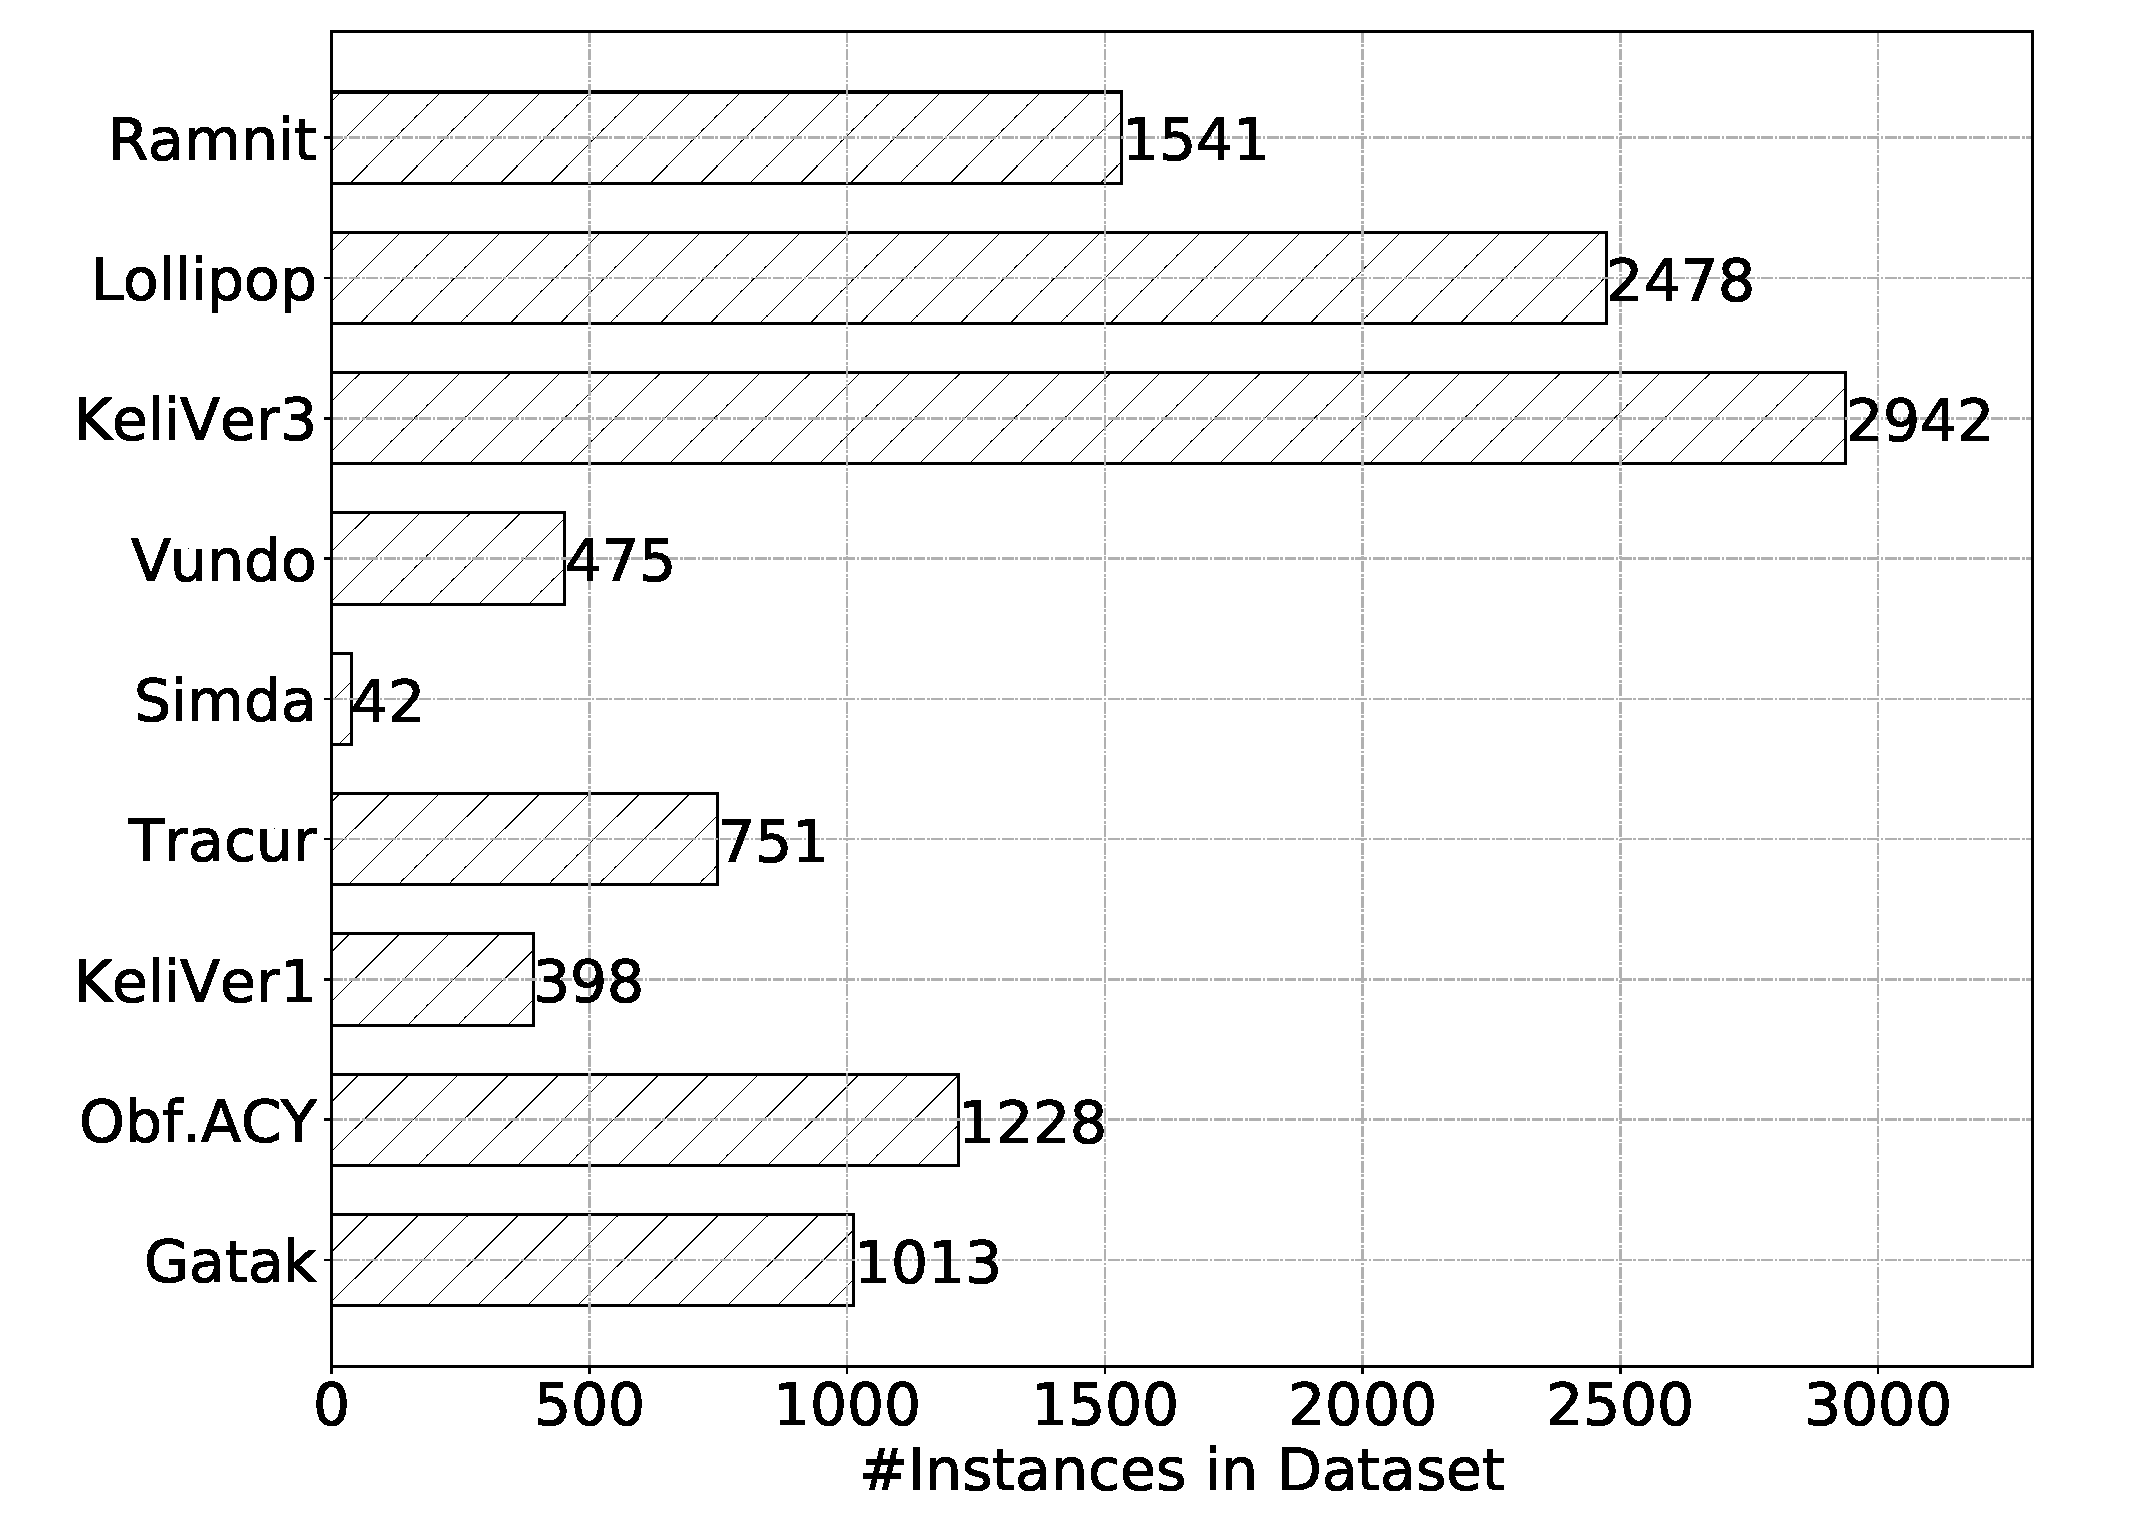
\includegraphics[width=0.44\textwidth]{Magic/figures/MsAcfgLabelDist.eps}}
\caption{Malware Family Distribution in MSKCFG Dataset.}
\label{MG:Fig:MSKCFGLabelDist}
\end{figure}

\begin{figure}
\centerline{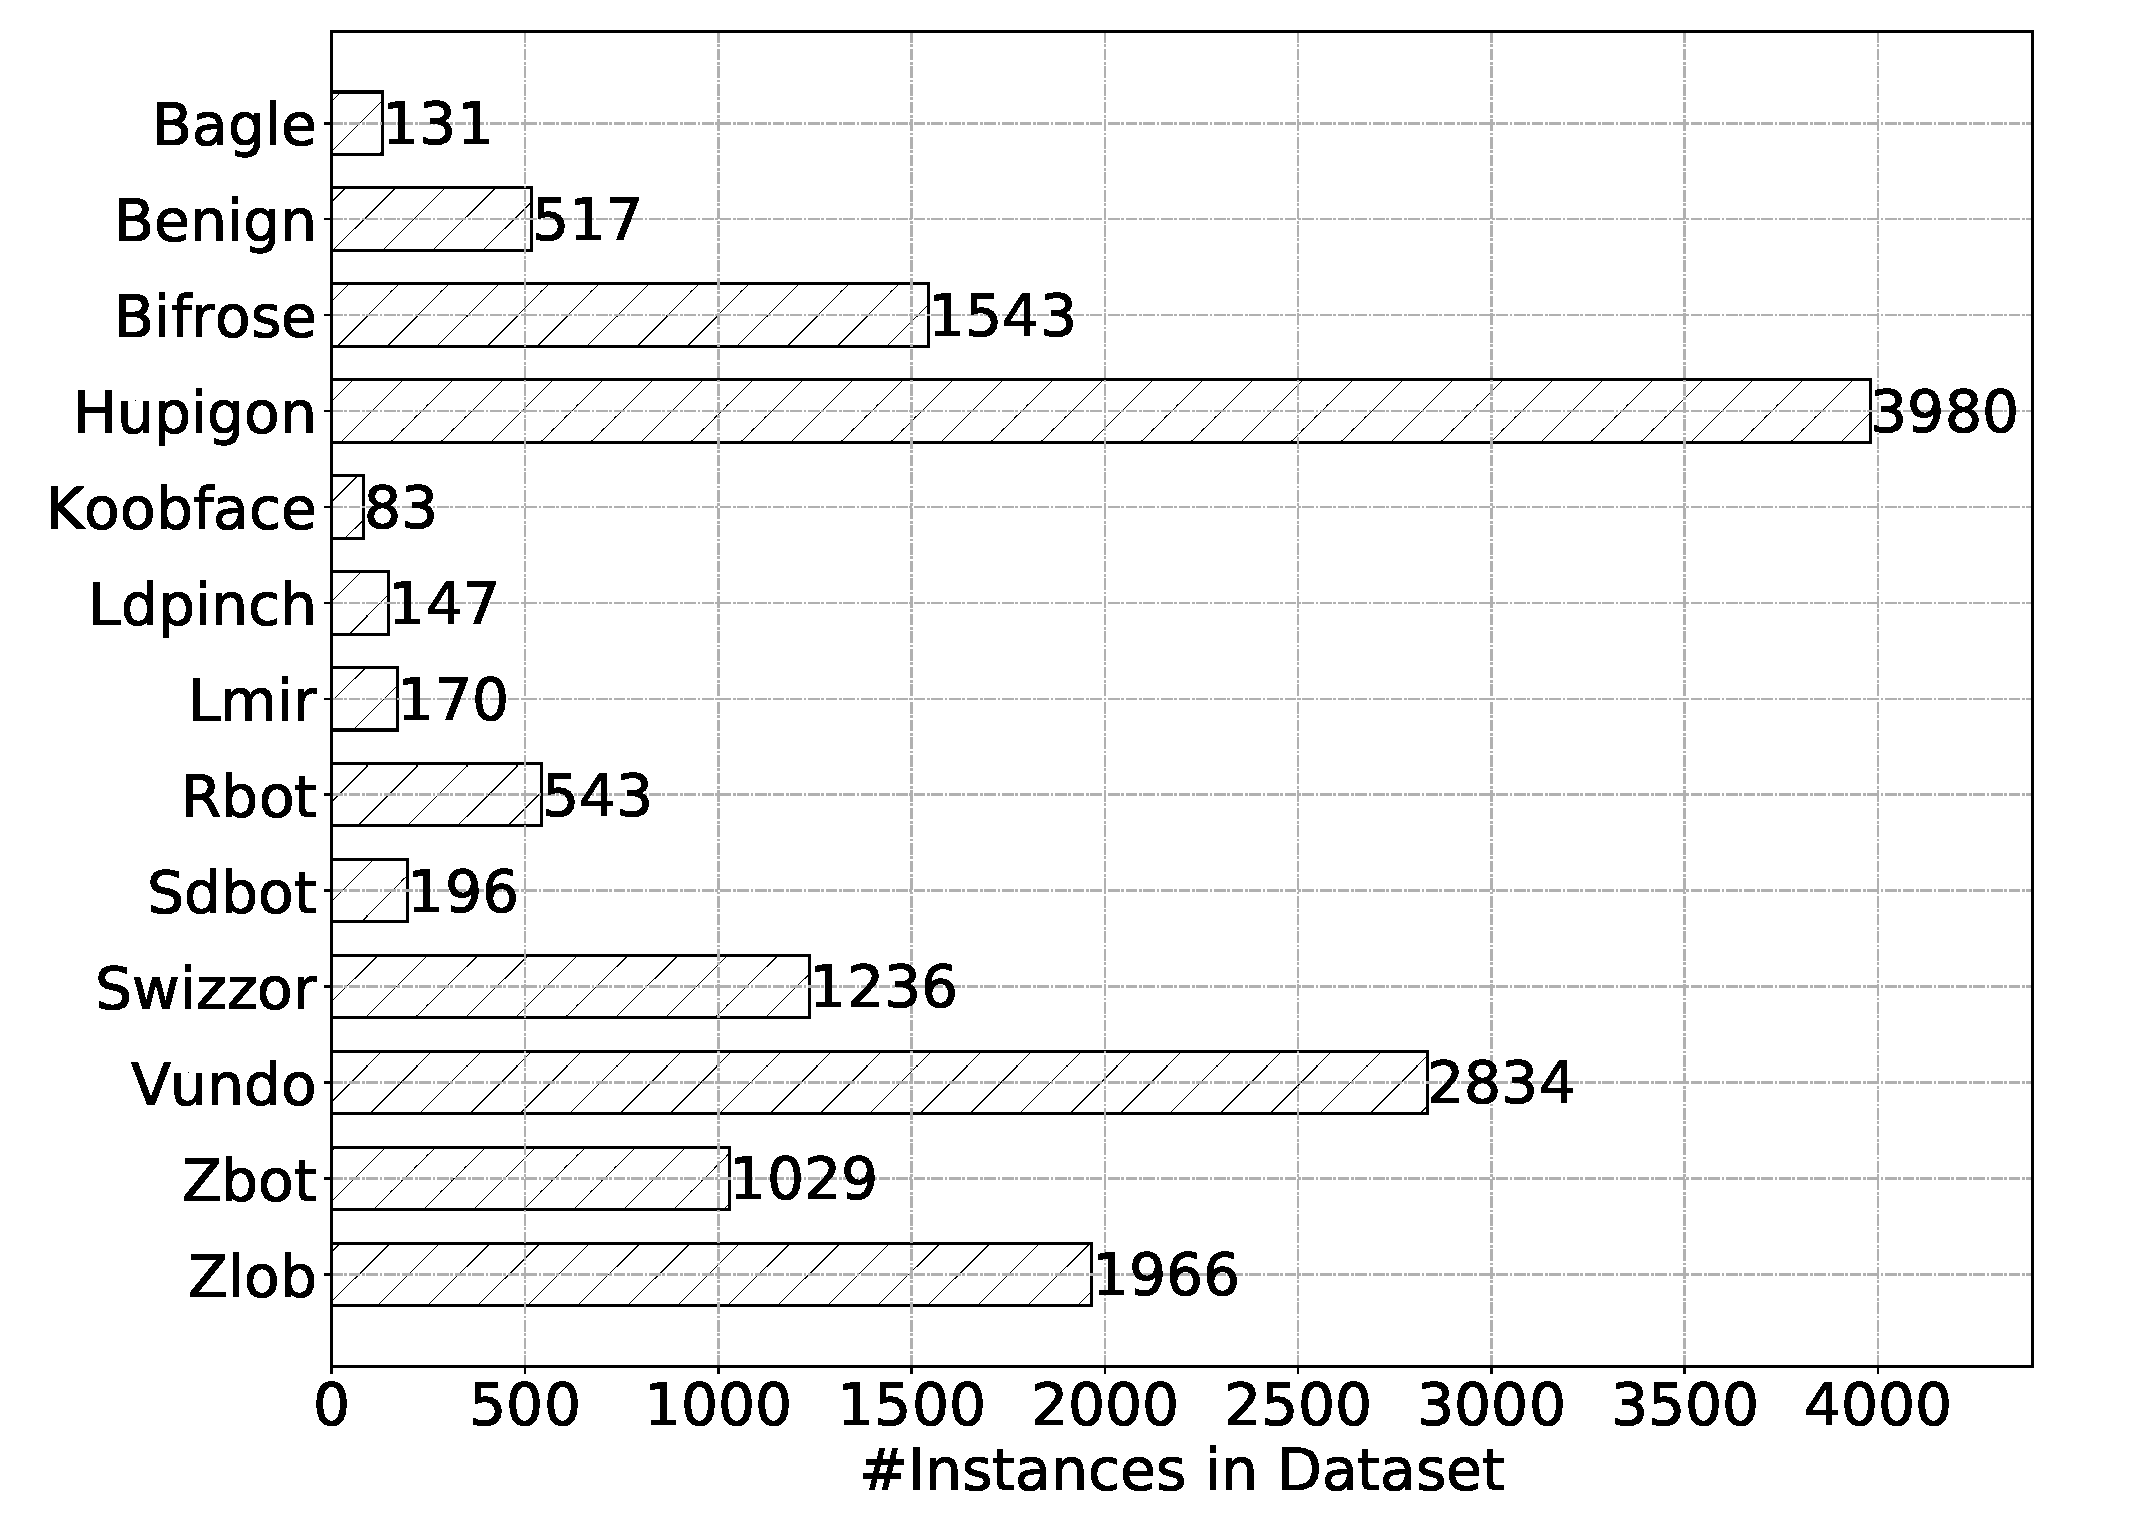
\includegraphics[width=0.44\textwidth]{Magic/figures/YanAcfgLabelDist.eps}}
\caption{Malware Family Distribution in YANCFG Dataset.}
\label{MG:Fig:YANCFGLabelDist}
\end{figure}

\subsection{Results on the MSKCFG Dataset}
The best cross-validation scores (precision, recall and F1) for the MSKCFG dataset are shown in Figure~\ref{MG:Fig:MSKCFGScores}, and the exact score values are listed in Table~\ref{MG:Tab:MSKCFGScores}.
The standard variances are not listed because the scores' variations among five different cross-validation folds are negligible ($<0.004$).
% Table~\ref{tab:MSKCFGConfusionMatrix} details the corresponding confusion table.
For all nine malware families, our best model has achieved good validation scores with precisions higher than 0.96, recalls higher than 0.96, and F1-scores higher than 0.97.

\begin{figure}
\centerline{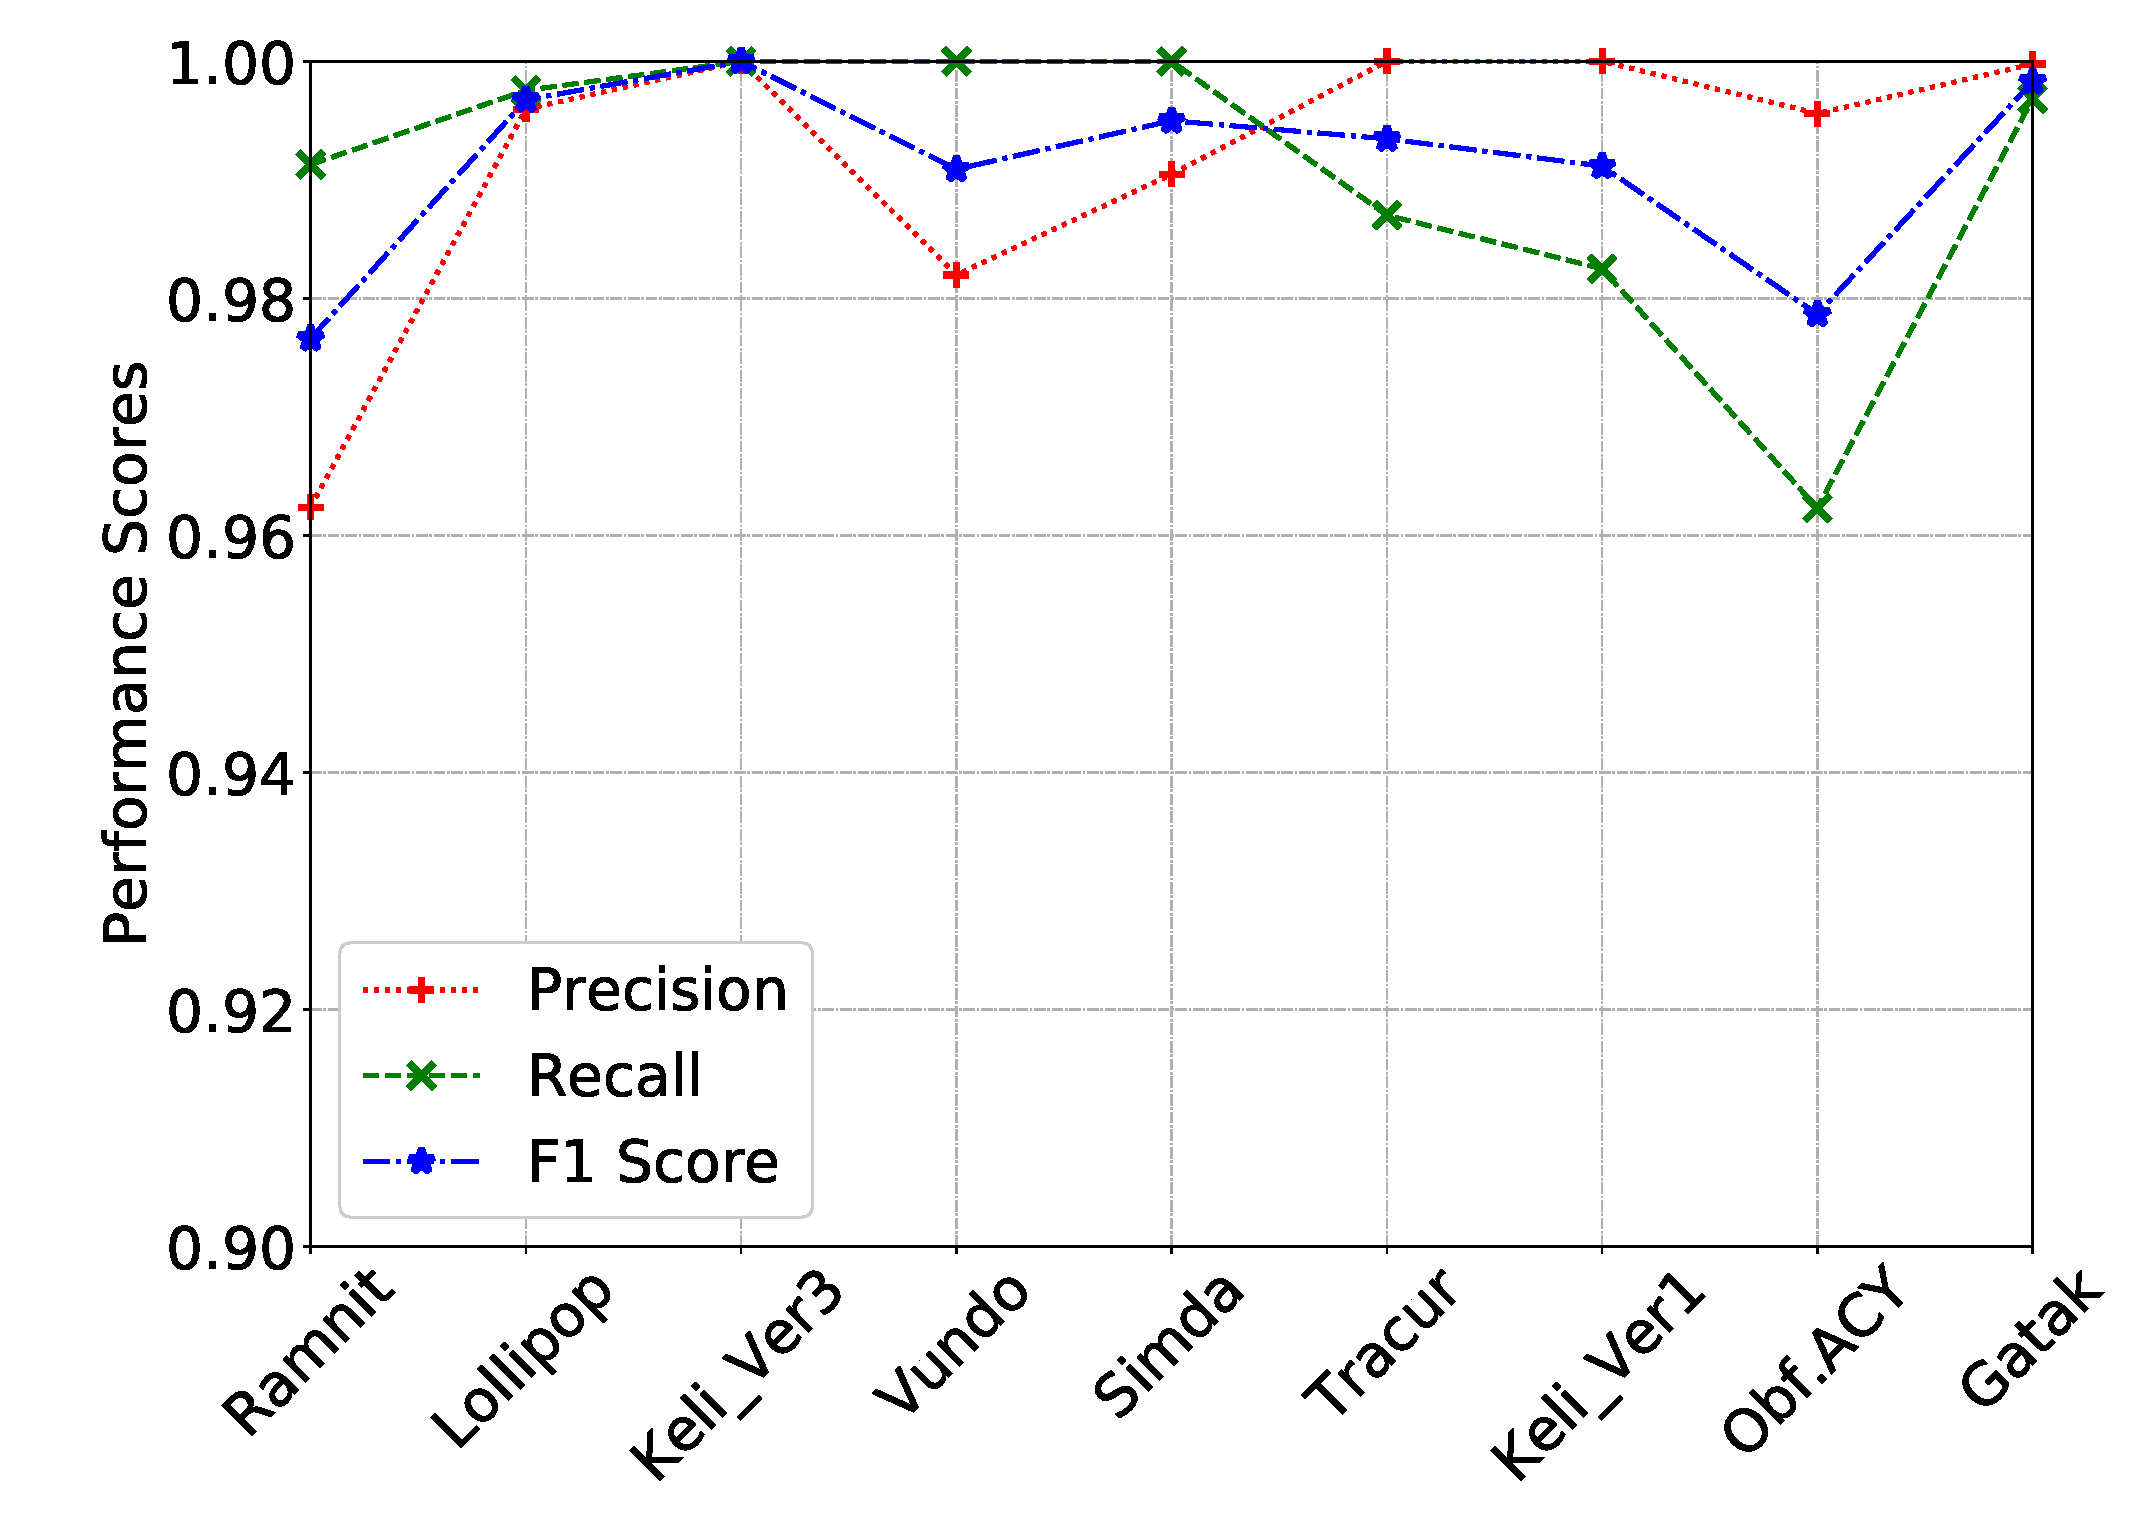
\includegraphics[width=0.44\textwidth]{Magic/figures/MsAcfgScores.eps}}
\caption{Cross-Validation Scores of \sysname on the MSKCFG Dataset.}
\label{MG:Fig:MSKCFGScores}
\end{figure}

\begin{table}
\caption{Performances of \sysname on the MSKCFG Dataset.}
\begin{center}
\begin{tabular}{l|rrr}
\hline
   Family       &  Precision &    Recall &        F1 \\
\hline
\hline
   Ramnit       &   0.962378 &  0.991289 &  0.976615 \\
 Lollipop       &   0.995960 &  0.997550 &  0.996754 \\
 Kelihos\_Ver3  &   1.000000 &  1.000000 &  1.000000 \\
    Vundo       &   0.981975 &  1.000000 &  0.990895 \\
    Simda       &   0.990476 &  1.000000 &  0.994987 \\
   Tracur       &   1.000000 &  0.987013 &  0.993463 \\
 Kelihos\_Ver1  &   1.000000 &  0.982493 &  0.991156 \\
Obfuscator.ACY  &   0.995593 &  0.962293 &  0.978655 \\
    Gatak       &   0.999775 &  0.996841 &  0.998304 \\
\hline
\end{tabular}
\end{center}
\label{MG:Tab:MSKCFGScores}
\end{table}

Since Microsoft released the competition dataset in 2015, many researchers have used the dataset (completely or partially) to evaluate their techniques for malware detection and classification~\cite{NovelFeatureFusion, EnsembleDNN, AutoEncoderMicrosoft, FunctionCallGraph, StaticFeatures, PolySeqCls, AutoEncoderFeatureLearn, YuxinMalwareDnn}.
We surveyed the works mentioned above and found that three of them cannot be directly compared with our results because they were using different metrics.
%and found that unfortunately every work either performed the evaluation in a unique way or gave their evaluation results using divided metrics due to varying reasons, making three works not directly comparable to ours. 
The works in \cite{EnsembleDNN} and \cite{YuxinMalwareDnn} used the Microsoft dataset in the context of \emph{malware detection}, where all the samples contained within it were treated as malicious, and then they were merged with a number of benign programs to construct a new dataset for malware detection.
As a result, their methods and performance metrics (two-class AUC, F1 score or accuracy) are not directly comparable to the approaches aimed at classifying malware samples into the corresponding families (e.g.,~\cite{NovelFeatureFusion, AutoEncoderMicrosoft, FunctionCallGraph, StaticFeatures, PolySeqCls, AutoEncoderFeatureLearn}), this work included. %, where models should predict the malware family that a sample belongs to.
Note that without loss of generality, benign software can be treated as a special family.
The work in~\cite{AutoEncoderMicrosoft} did not adopt the cross-validation methodology. Instead, the authors manually split the training dataset into 75\% training data and 25\% holdout testing data, and reported the mean square error, accuracy and confusion matrix over both training and testing data.
The holdout set is not the test set provided by Microsoft. 
Therefore, we did not compare our work with the evaluation results reported in \cite{EnsembleDNN}, \cite{YuxinMalwareDnn} and \cite{AutoEncoderMicrosoft}.

Among the other five papers of malware classification, both \cite{FunctionCallGraph} and \cite{StaticFeatures} conducted the ten-fold cross validation over the Microsoft dataset, but only reported the overall accuracy.
\cite{PolySeqCls} also performed a ten-fold cross validation but reported both the overall accuracy and logarithmic loss.
Both \cite{NovelFeatureFusion} and \cite{AutoEncoderFeatureLearn} performed a five-fold cross validation and reported both the overall accuracy and logarithmic loss.
Since the Microsoft dataset is not balanced across malware families, we compare \sysname with the five previous works that reported not only the overall accuracy but also the mean logarithmic loss, and the results are shown in Table~\ref{MG:Tab:CompareMicrosoftCv}.

The methods listed in Table~\ref{MG:Tab:CompareMicrosoftCv} can be classified into either ensemble-learning or single-model based approaches.
\cite{NovelFeatureFusion} extracts more than 1800 features and uses gradient boosting based classifier, and it achieves the best log-loss (0.0197) and accuracy (99.42\%) using the XGBoost classifier. 
\cite{FunctionCallGraph} achieves the second best accuracy (99.3\%) by ensembling multiple random forest methods, which already ensembles multiple decision trees.
The DGCNN-based technique used by MAGIC achieves highly competitive results.
In fact, the logarithmic loss (0.0543) is the second best; the accuracy (99.25\%) is the third best, only 0.005 less than the second best one (99.3\% reported by \cite{FunctionCallGraph}).
\cite{AutoEncoderFeatureLearn} adopts a deep-learning based hybrid approach.
It relies on a single deep autoencoder to perform automatic feature learning, and then uses gradient-boosting based classifier to make the prediction.
As an alternative work that also applies deep neural network, our DGCNN-based approach outperforms the work in~\cite{AutoEncoderFeatureLearn} by 27.40\% in terms of logarithmic loss and 1.5\% in terms of classification accuracy.
%regarding log-loss (27.40\% improvement) and accuracy (1.5\% improvement).

\begin{table*}
\caption{Cross Validation Metric Comparison on the Microsoft Dataset.}
\begin{center}
\begin{tabular}{l|rr}
\hline
   Approach Brief Description                                           & Mean Logarithmic Loss     & Accuracy \\
\hline
\hline
\sysname                                                                &               0.0543      &   99.25 \\
XGBoost with Heavy Feature Engineering\cite{NovelFeatureFusion}         &               0.0197      &   99.42 \\
Deep Autoencoder based XGBoost\cite{AutoEncoderFeatureLearn}            &               0.0748      &   98.20 \\
Strand Gene Sequence Classifier\cite{PolySeqCls}                        &               0.2228      &   97.41 \\
Ensemble Multiple Random Forest Classifiers\cite{FunctionCallGraph}     &       Not Reported        &   99.30 \\
Random Forest with Feature Engineering\cite{StaticFeatures}             &       Not Reported        &   99.21 \\
\hline
\end{tabular}
\end{center}
\label{MG:Tab:CompareMicrosoftCv}
\end{table*}


% \begin{table*}
% \centering
% \caption{Confusion Matrix on the MSKCFG Dataset}
% \begin{tabular}{l|rrrrrrrrr}
%   Family       &  Ramnit &  Lollipop & Kelihos\_Ver3 &  Vundo &  Simda &  Tracur & Kelihos\_Ver1 & Obfuscator.ACY &  Gatak \\
% \hline
% \hline
%    Ramnit       &     321 &         2 &             0 &      0 &      0 &       2 &             0 &              3 &      0 \\
%  Lollipop       &       4 &       443 &             0 &      0 &      0 &       0 &             0 &              0 &      0 \\
% Kelihos\_Ver3   &       0 &         0 &           586 &      0 &      0 &       0 &             0 &              0 &      0 \\
%     Vundo       &       0 &         0 &             0 &     88 &      0 &       0 &             0 &              0 &      0 \\
%     Simda       &       0 &         1 &             0 &      0 &      8 &       0 &             0 &              0 &      0 \\
%    Tracur       &       1 &         1 &             0 &      0 &      0 &     174 &             0 &              0 &      0 \\
% Kelihos\_Ver1   &       0 &         0 &             0 &      3 &      0 &       0 &            65 &              0 &      0 \\
% Obfuscator.ACY  &       9 &         1 &             0 &      0 &      0 &       0 &             0 &            235 &      0 \\
%     Gatak       &       0 &         0 &             0 &      1 &      0 &       0 &             0 &              0 &    210 \\
% \end{tabular}
% \label{MG:Tab:MSKCFGConfusionMatrix}
% \end{table*}


\subsection{Results on the YANCFG Dataset}
\sysname's best cross validation scores on the YANCFG dataset are depicted in Figure~\ref{MG:Fig:YANCFGScores} and the exact values of these scores are listed in Table~\ref{MG:Tab:YANCFGScores}.
% Table~\ref{tab:YANCFGScores} is the corresponding confusion table on the 20\% holdout set.
We observe in Figure~\ref{MG:Fig:YANCFGScores} that \sysname achieves F1-scores higher than 0.9 for nine of the 13 binary families including \{Bagle, Benign, Bifrose, Hupigon, Koobface, Swizzor, Vundo, Zbot, Zlob\}.
The classification performances on both the Koobface and Swizzor families are perfect with a precision of 1.0 and a recall of 1.0.
Regarding the other five families with F1 scores lower than 0.8, they all have relatively small populations in the YANCFG dataset.
Our classifier suffers relatively low recalls (around 0.5) for both the Ldpinch and Sdbot families. For the Ldpinch, Rbot and Sdbot families, their precision scores (between 0.64 and 0.70) are not as good as the other ten families (more than 0.8).

In order to further assess \sysname, we compared our results to the F1 scores obtained in~\cite{YanDataset}.
That work ensembles a group of individual SVM (Support Vector Machine)-based classifiers (refer to \textbf{ESVC} hereafter). Our work does not use the raw hexadecimal bytes, the PE headers, and the execution traces in the original dataset.%, which put our approach at a disadvantage.
We plot the comparison results in Figure~\ref{MG:Fig:YANCFGF1Improve} as the relative and absolute amount of improvement to ESVC as achieved by \sysname.
Note that the improvement statistics for the Benign family are not shown in Figure~\ref{MG:Fig:YANCFGF1Improve} because the F1 score for the benign samples is not reported in~\cite{YanDataset}.
The positive values in Figure~\ref{MG:Fig:YANCFGF1Improve} mean factual improvement, while the negative values mean degradation.
Close to the bottom of the figure, we observe that the only family over which \sysname performs visibly poorer than ESVC is Rbot, with an approximate performance degradation of 0.07 relatively and 0.05 absolutely.
For Hupigon, the downgradation is nearly invisible (less than 0.01 both relatively and absolutely), and both approaches achieve F1 scores higher than 0.94.
On the other hand, \sysname outperforms ESVC for the other ten families.
Moreover, the amount of absolute improvement is greater than or equal to 0.2 for each of the Bagle, Koofbace, Ldpinch and Lmir families.
Lastly, it is noted that both approaches performed relatively poorly on the Ldpinch and Lmir malware families. Still, the DGCNN-based approach used by \sysname improves the work in \cite{YanDataset} by 70\% and 35\% in terms of the F1-score for Ldpinch and Lmir, respectively.


\subsection{Discussion}
% We break down the major execution overhead of \sysname, XGBoost\cite{NovelFeatureFusion}, and ESVC\cite{YanDataset} into three parts: feature extraction time, classifier training time, and malware prediction time.
% In order to extract 1,804 features from both byte code files and disassembled code, it takes XGBoost\cite{NovelFeatureFusion} around 48 hours (173,264 seconds) to process the entire MSKCFG dataset on a laptop with a quad-core 2 GHz and 8GB RAM.
% In contrast, building ACFGs for the MSKCFG dataset with MAGIC takes around 17 hours. %, as mentioned at the beginning of this section. 
% The execution time spent on feature collection and extraction was not mentioned in \cite{YanDataset}.

We break down the major execution overhead of \sysname into three parts: feature extraction time, classifier training time, and malware prediction time.
Building ACFGs for the MSKCFG dataset with MAGIC takes less than 6 seconds on average.
We gathered the training and testing running time over 20 runs to evaluate \sysname.
% The training and prediction overhead is not reported in~\cite{NovelFeatureFusion}.
% In the experiments conducted in~\cite{YanDataset}, the mean malware prediction time per instance is around 278 milliseconds.
% In our experiments using \sysname
The mean and standard deviation of the classifier training time per instance among the 20 runs is approximately 29.69$\pm$4.90 milliseconds,
while the mean and standard deviation of malware prediction time per instance is only 11.33$\pm1.35$ milliseconds.
% Moreover, the size of the trained DGCNN model in \sysname is around 420 MB.
Our measurements of the execution overhead of \sysname suggest that it is actionable for online malware classification in practice.
%Although the execution performances mentioned above were measured on different machines, we believe that \sysname is actionable in practice for online malware classification due to its low execution overhead.

By design, \sysname is aimed at striking a balance between generality and performance.
XGBoost~\cite{NovelFeatureFusion} achieves impressive performance (99.42\% CV accuracy for MSKCFG), but relies on various handcrafted features (more than 1800 from the MSKCFG dataset) and time-consuming feature selection techniques (e.g., forward stepwise selection).
In contrast, \sysname achieves a similar performance (99.25\%) with only a dozen easy-to-extract attributes embedded within malware’s CFG structures.
The work in~\cite{YanDataset} sequentially integrates SVM-based malware classifiers trained from heterogeneous features,
but its use of dynamic programming to search an optimal malware classifier with a bounded false positive rate increases model training time significantly.

The YANCFG and MSKCFG datasets are the two largest labeled malware datasets that we could obtain to evaluate our work.
It is possible that malware development trends after the collection of these two datasets introduce new challenges to the malware classification problem.
We plan to test our models with the latest malware samples in our future work.


\begin{table}
\caption{Performance of \sysname on the YANCFG Dataset.}
\begin{center}
\begin{tabular}{l|rrr}
\hline
   Family &  Precision &    Recall &  F1 Score \\
\hline
\hline
    Bagle &   0.863636 &  0.950000 &  0.904762 \\
   Benign &   0.954128 &  0.962963 &  0.958525 \\
  Bifrose &   0.930380 &  0.901840 &  0.915888 \\
  Hupigon &   0.935287 &  0.945679 &  0.940454 \\
 Koobface &   1.000000 &  1.000000 &  1.000000 \\
  Ldpinch &   0.692308 &  0.514286 &  0.590164 \\
     Lmir &   0.833333 &  0.731707 &  0.779220 \\
     Rbot &   0.641221 &  0.763636 &  0.697095 \\
    Sdbot &   0.700000 &  0.488372 &  0.575342 \\
  Swizzor &   0.995708 &  0.995708 &  0.995708 \\
    Vundo &   0.990859 &  0.981884 &  0.986351 \\
     Zbot &   0.941799 &  0.936842 &  0.939314 \\
     Zlob &   0.967254 &  0.992248 &  0.979592 \\
\hline
\end{tabular}
\end{center}
\label{MG:Tab:YANCFGScores}
\end{table}

\begin{figure}
\centerline{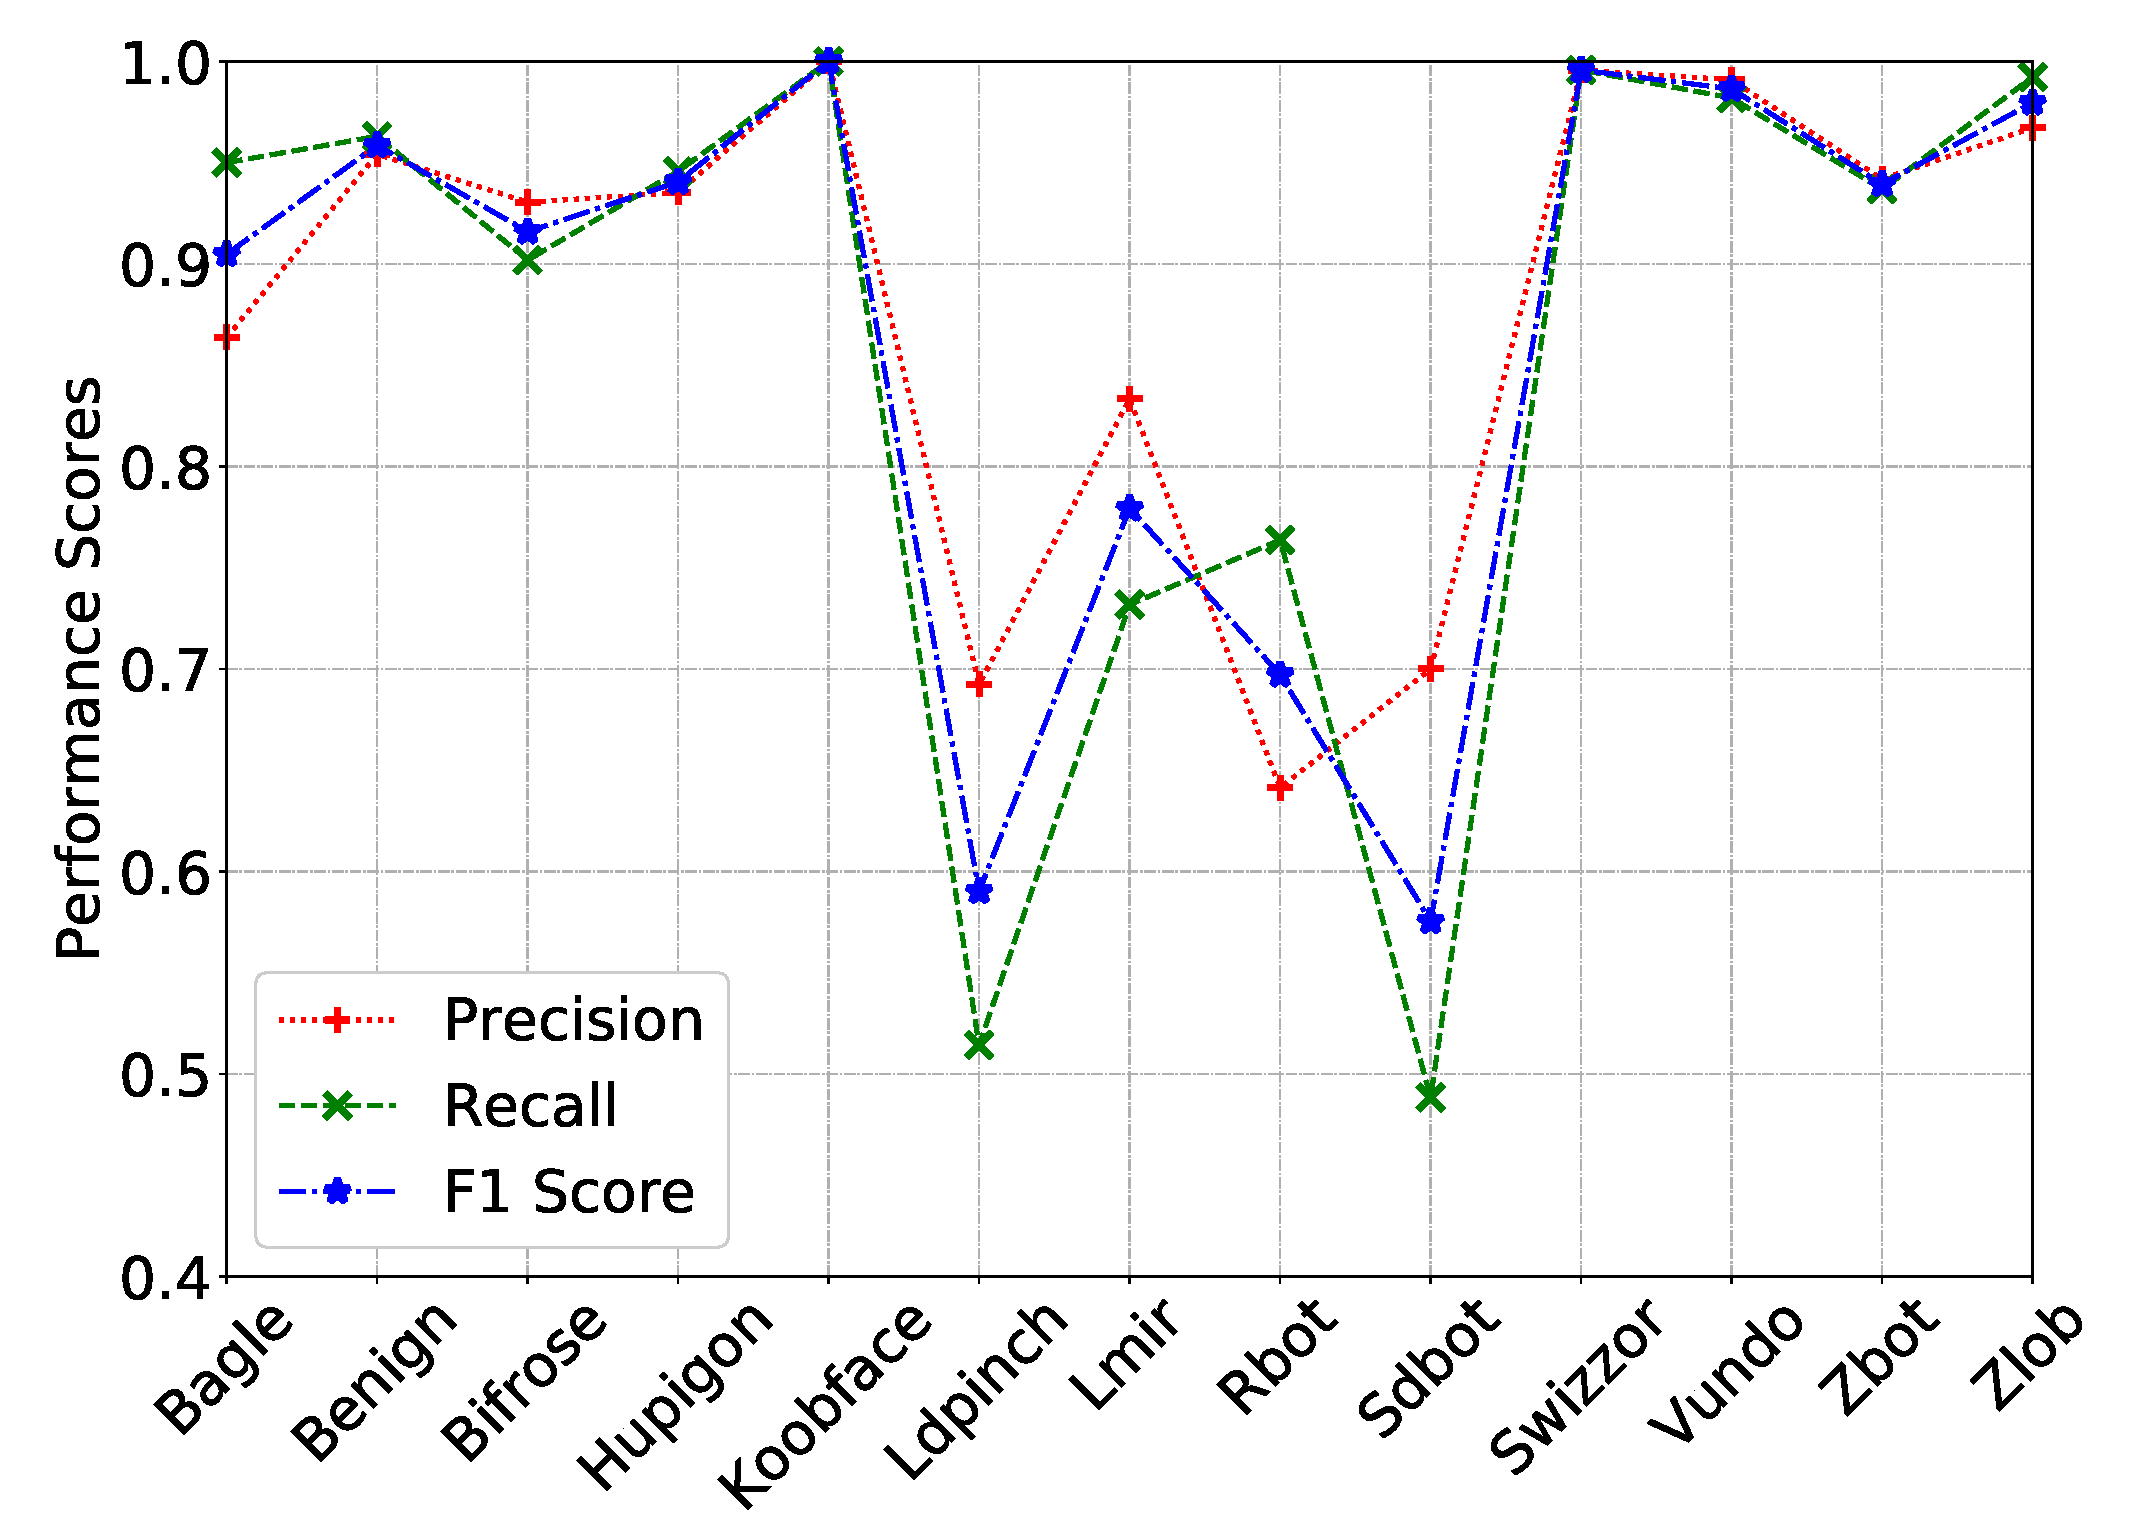
\includegraphics[width=0.48\textwidth]{Magic/figures/YanAcfgScores.eps}}
\caption{Cross-Validation Scores of \sysname on the YANCFG Dataset.}
\label{MG:Fig:YANCFGScores}
\end{figure}

\begin{figure}
\centerline{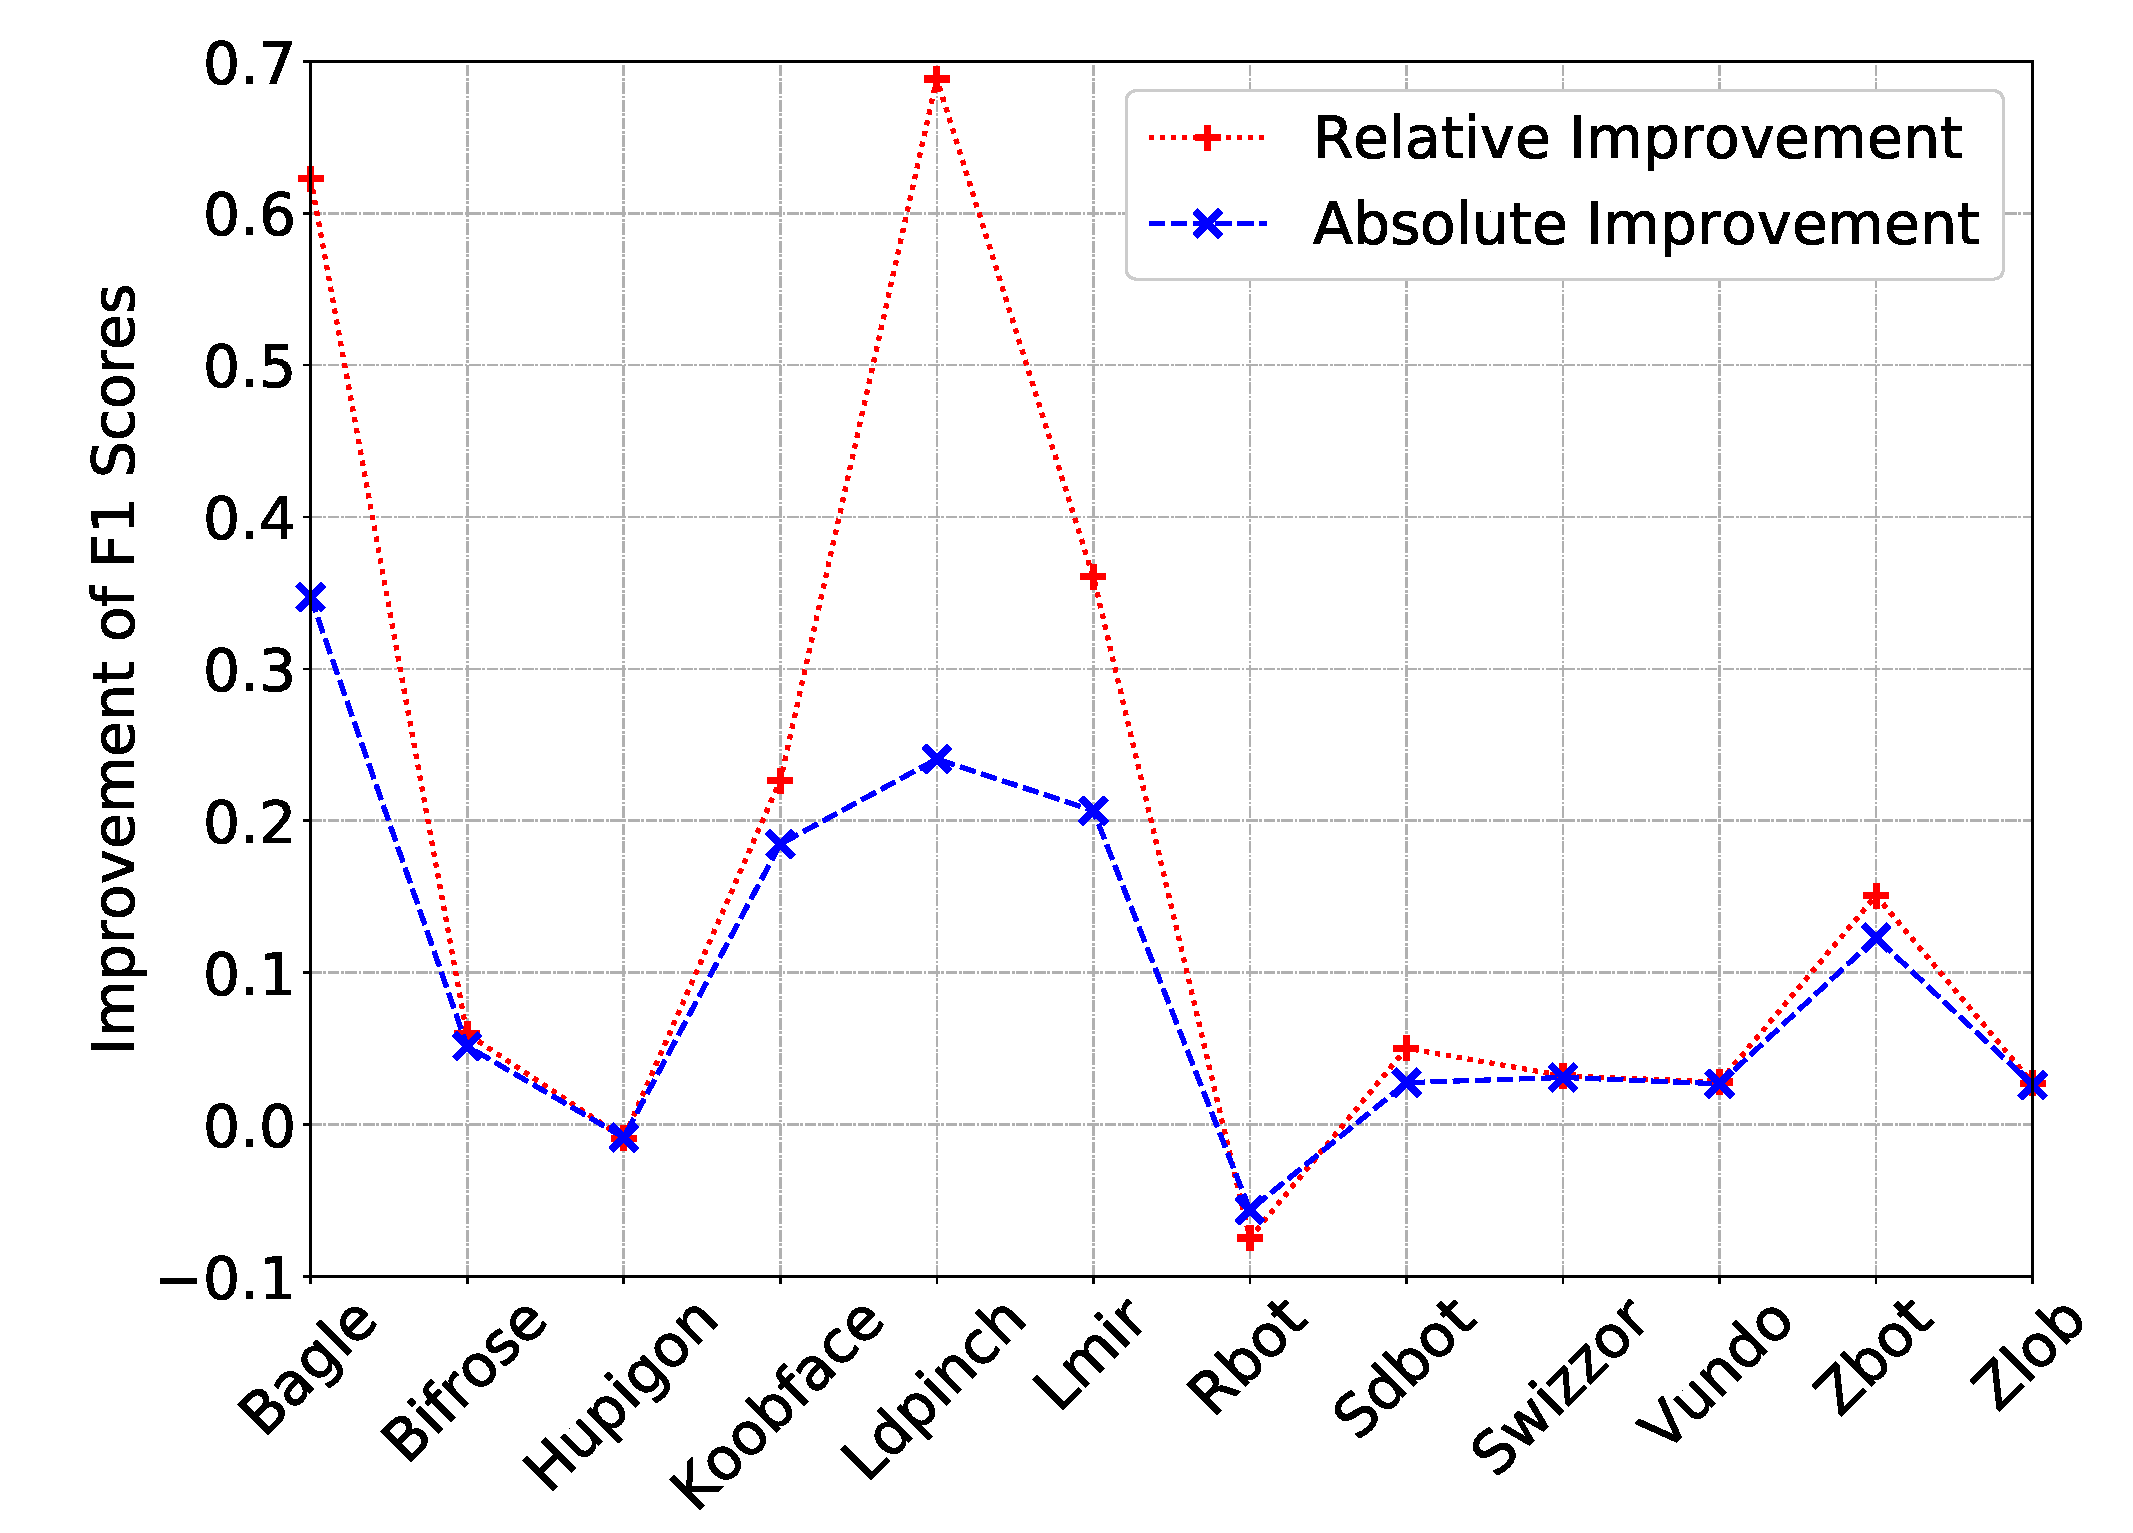
\includegraphics[width=0.48\textwidth]{Magic/figures/YanAcfgF1Improve.eps}}
\caption{F1 Score Comparison between \sysname and ESVC\cite{YanDataset} on the YANCFG Dataset.
Improvement on the classification accuracy of benign samples is not shown because it is not reported in \cite{YanDataset}.}
\label{MG:Fig:YANCFGF1Improve}
\end{figure}

% \begin{table*}
% \centering
% \caption{Confusion Matrix on the YANCFG Dataset}
% \begin{tabular}{l|rrrrrrrrrrrrr}
%   Family &  Bagle &  Benign &  Bifrose &  Hupigon &  Koobface &  Ldpinch &  Lmir &  Rbot &  Sdbot &  Swizzor &  Vundo &  Zbot &  Zlob \\
% \hline
% \hline
%     Bagle &     19 &       0 &        0 &        0 &         0 &        0 &     0 &     1 &      0 &        0 &      0 &     0 &     0 \\
%    Benign &      0 &     104 &        1 &        1 &         0 &        0 &     0 &     0 &      0 &        1 &      0 &     0 &     1 \\
%   Bifrose &      0 &       2 &      294 &       14 &         0 &        3 &     2 &     8 &      1 &        0 &      1 &     0 &     1 \\
%   Hupigon &      1 &       0 &        8 &      766 &         0 &        0 &     3 &    18 &      6 &        0 &      3 &     5 &     0 \\
%  Koobface &      0 &       0 &        0 &        0 &        20 &        0 &     0 &     0 &      0 &        0 &      0 &     0 &     0 \\
%   Ldpinch &      2 &       0 &        2 &        6 &         0 &       18 &     0 &     4 &      0 &        0 &      0 &     3 &     0 \\
%      Lmir &      0 &       2 &        0 &        7 &         0 &        1 &    30 &     1 &      0 &        0 &      0 &     0 &     0 \\
%      Rbot &      0 &       0 &        5 &       16 &         0 &        0 &     1 &    84 &      2 &        0 &      0 &     1 &     1 \\
%     Sdbot &      0 &       1 &        2 &        4 &         0 &        2 &     0 &    12 &     21 &        0 &      0 &     1 &     0 \\
%   Swizzor &      0 &       0 &        0 &        1 &         0 &        0 &     0 &     0 &      0 &      232 &      0 &     0 &     0 \\
%     Vundo &      0 &       0 &        3 &        1 &         0 &        0 &     0 &     1 &      0 &        0 &    542 &     0 &     5 \\
%      Zbot &      0 &       0 &        1 &        3 &         0 &        1 &     0 &     1 &      0 &        0 &      1 &   178 &     5 \\
%      Zlob &      0 &       0 &        0 &        0 &         0 &        1 &     0 &     1 &      0 &        0 &      0 &     1 &   384 \\
% \end{tabular}
% \label{MG:Tab:YANCFGConfusionMatrix}
% \end{table*}


% We introduce related works on deep learning based malware classification and deep neural networks for graph data.

% \subsection{Weakness of Existing Malware Detection Approaches}
% In the solution that wins the 2015 Microsoft Malware Classification Challenge\cite{MsWinner}, one set of useful features are the intensities of the first 800 pixels.
% While viewing malware binary as gray-scale images make some sense in some ways and was adopted by a number of existing classification methods,
% why care about the first 800 pixels' intensities in particular, say why not 400?
% Some existing approaches\cite{GraphMalwareDetect, QgramMalwareDetect} require collecting execution traces of the in-question executable;
% this is also impossible if the given PE-header is stripped.
% As in the Microsoft Malware Classification Challenge case,
% malware developers can easily counter the first-800-pixel-intensity features by padding certain pixels that statistically close to these in normal binaries.
% Similar mechanism can be conveniently employed to confuse the detection approaches that heavily relies on opcode n-grams\cite{NgramMalwareDetect, QgramMalwareDetect, McBoost}.

\section{Deep Learning Based Malware Detection}

As an important problem in cybersecurity, malware detection and classification have drawn the attentions of many researchers from both communities of cybersecurity and data mining~\cite{MalDetectSurvey1, MalDetectSurvey2}.
There has been a recent trend of applying deep learning techniques for malware defense tasks and these works largely fall into two categories.
In the first category, which adopts a feature-centric approach, researchers reuse or extend features developed in previous works but extracted from the newer datasets collected from customized, private, and specific environments~\cite{EarlyStageRnn, DeepFlow, DeepAM, RandomProjectionNn, AutoEncoderFeatureLearn, AutoEncoderMicrosoft, LstmSyscall, MalwareLstmGru}.
For example, the work in~\cite{DeepFlow} focused on malware collected from Android devices and that in~\cite{DeepAM} targets malware on the cloud platforms.
Off-the-shelf deep learning models have been used as tunable black boxes.
Compared with classic machine learning algorithms like decision trees, random forest, and gradient boosting,
deep learning models fed with the same training datasets may result in better detection performance~\cite{DeepFlow,RandomProjectionNn} and faster execution~\cite{EarlyStageRnn},
because of their advantages on big data analysis~\cite{RandomProjectionNn} and the possibility of using parallel computing hardware (i.e., GPUs).
Moreover, the works in~\cite{AutoEncoderFeatureLearn} and~\cite{AutoEncoderMicrosoft} have focused on automation of feature learning using unsupervised deep learning techniques.

In the second category, which adopts a model-centric approach, researchers are motivated by finding specific but superior deep learning architectures for malware defense tasks.
For example, to find similar success of convolution neural network in the application domains of computer vision and image classification, researchers have proposed methods to transform the byte sequences in binary malware executables into gray or color images, which are amenable to the existing deep learning-based image classification techniques~\cite{R2D2, GibertCnn}. Other researchers have explored how deep sequence models, such as LSTM, GRU, and the attention mechanism, can be applied to programs the sequences of system calls or API calls transformed from malware programs~\cite{LstmSyscall,MalwareLstmGru}. 

%Many existing works including our work that apply deep learning to malware detection is a hybrid of the two categories.
Our work takes a hybrid approach that intersects with the works in both categories. First, our work improves the accuracy of malware classification using not only the features that can be explicitly expressed with numeric values (i.e., attributes extracted from basic blocks) but also those that are inherent within the structure of the program (i.e., control flow graphs). On the other hand, deep learning models are not used as black boxes in our work, as we have proposed modifications to the standard DGCNN that are better tailored to the malware classification problem.

\section{Deep Learning Models for Graph-Represented Data}

%As people in today's world are increasingly connected by computer network and social network, data collected from our digital lives are also organized in networks or graphs.
%Motivated by the increasingly available graphical datasets, researchers in artificial intelligence and data science community are studying how neural network can help computers to efficiently learn the inherent relationships that reside in graph's unordered connectivity.
There are two parallel lines of research on deep learning algorithms for graph-represented data.
In the first setting~\cite{Node2Vec, LineNetworkEmbedding, SemiSupervisedGcn}, a single graph is given and the task is to infer unknown labels of individual vertices, or  unknown types of connectivity between vertices.
Though this problem has wide applications in social networks and recommendation systems, it does not align well with our goal in this paper. 
Instead, our work fits into the second setting, where assuming a group of labeled graphs with different structures and sizes, the task is to predict the label of future unknown graphs\cite{Dgcnn, SeqGraphKernels, SimonovskyEcc}.
In this setting, both the works in~\cite{SeqGraphKernels} and~\cite{Dgcnn} have mentioned their connections with the classic Weisfeiler-Lehman subtree kernel~\cite{WlGraphKernel} or the Weisfeiler-Lehman algorithm~\cite{WlAlgorithm}.
In contrast, the work in~\cite{SeqGraphKernels} introduces the recurrent neuron based graph kernel, then stacks multiple graph kernel neural layers into deep network.
Similar to the sort pooling layer discussed in~\cite{Dgcnn}, the work in~\cite{SimonovskyEcc} generalizes the convolution operator and enables it to handle arbitrary graphs of different sizes.
In our work, we propose to enhance the architectures introduced in~\cite{Dgcnn} with both the weight vertices layer and the adaptive max pooling layer for the malware classification task.


\Chapter{Conclusion}
\label{Sec:Conclusion}

\section{Summary of Current Work}

Under the centre theme of securing SDN-enabled large-scale network using high-fidelity and scalable testing system, we conduct our research work in three streams.
First, we address one of the key issues in Linux-container-based network emulation (LCNE).
Even though LCNE combines many desired features of software simulation and physical testbeds,
it uses the system clock across all the containers even if a container is not being scheduled to run.
This leads to the issue of both performance and temporal fidelity, especially with high workloads.
Virtual time sheds the light on this issue by precisely scaling the time of interactions between containers and physical devices.
We develope a lightweight Linux-container-based virtual time system and integrate it to Mininet.
Except for enhancing Minint's fidelity and scalability,
our virtual time system is also an alternative for synchronizing clocks in hybrid simulation and emulation.
Second, we rethink how to simulate SDN network by taking advantage of the centralized paradigm.
Following this idea, we present a model abstraction technique that effectively transforms
the network devices in an SDN-based network to one virtualized switch model.
While significantly reducing the model execution time and enabling the real-time simulation capability,
our abstracted model also preserves the end-to-end forwarding behavior of the original network.
Third, motivated by the recent advancement and success of deep neural networks,
we study the feasibility of deep learning based network intrusion detection systems (NIDS) in order to enhance the essential network-architecture-agnostic security building-block.
We construct the detection engine with multiple advanced deep learning models and compare their performance.

\section{Future Work}
Malware detection with executable is promising
\cite{GatedConvNet, ACFG4BugSearch, GraphEmbedSimDetection, MalConvNvidia}.
%When applying the machine learning algorithms or design customized neural networks, the following
%should be taken into consideration as guidance:
%\begin{enumerate}
%\item The informative PE header of a particular Windows OS, is well-defined and also complicated.
        %Minimal domain knowledge should be relied on since they are fragile;
        %the author of the malware may intentionally leverage these rules to hide key part of the malicious code.
%\item There are high amount of positional variation presented in the executable files.
    %Since PE header 
%\end{enumerate}

\begin{algorithm}[h]
\DontPrintSemicolon
    \KwIn
    {
        $D = $ binary code dataset. \newline
        $bc = $ a particular binary code file in $D$. \newline
        $g \equiv (V, E, x) = ACFG(bc) $ the ACFG of a particular binary code file. \newline
        $\mu_v = $ feature vector of a particular node in ACFG. \newline
        $nn \equiv $ neural network with parameters $W_1, P_1, P_2, W_2$.
    }
    \SetKwProg{Fn}{Function}{}{\KwRet}
    \SetKwFunction{ACFG}{acfg\_bytecode}
    \SetKwFunction{EmbeddingACFG}{embedding\_acfg}
    \SetKwFunction{GetBatchEmbedding}{get\_batch\_embedding}
    \SetKwFunction{Train}{train}
    \Fn{\EmbeddingACFG{$g$, $nn$}} {
        Algorithm 1 in paper\;
        But return the set of vertex embeddings $\mu_g = \{\mu_v| \forall v \in V\}$\;
    }
    \Fn{\GetBatchEmbedding{$nn$}} {
        $batch\_ACFG= $ sample $batch\_size$ binary code files from $D\_ACFG$\;
        Pair $g \in batch\_ACFG$ with 1 positive and 1 negative ACFG to obtain
        $batch\_pairs = {(g_i, g_j, 1), (g_i, g_j', -1) | g_i \in batch\_ACFG}$\;
        \ForEach (// Embed $batch\_pairs$ to $batch\_embeddings$) {$(g_i, g_j, label) \in batch\_pairs$} 
        {
            $\mu_{g_i}$ = \EmbeddingACFG{$g_i$, $nn$}\;
            $\mu_{g_j}$ = \EmbeddingACFG{$g_j$, $nn$}\;
            Append $(\mu_{g_i}, \mu_{g_j}, label)$ to $batch\_embeddings$\;
        }
        \KwRet{$batch\_embeddings$}
    }
    \Fn{\Train{$D$}} {
        Initialize parameters in $nn$\;
        Convert all byte code files: $D\_{ACFG} = \{ g | g = $ \ACFG{$bc$} $\forall bc \in D\}$\;
        \For (// Train $E$ epochs) {epoch = 1 to 100} {
            \For (// Train with batch data) {i = 1 to $\frac{||D||}{batch\_size}$} {
                $batch\_embeddings = $ \GetBatchEmbedding{$nn$}\;
                $nn$.fit($batch\_embeddings$)\;
            }
        }
    }
\caption{End-to-End Traning Algorithm with Embedding}
\end{algorithm}


\section*{Acknowledgment}
We would like to thank the anonymous DSN reviewers and our shepherd Long Wang for their valuable feedback.
We also thank Ping Liu for the insightful discussions and Muhan Zhang for the bug fixes in the pytorch version of DGCNN.
This work is partly sponsored by the Air Force Office of Scientific Research (AFOSR) under Grant YIP FA9550-17-1-0240,
the National Science Foundation (NSF) under Grant CNS-1618631, and the Maryland Procurement Office under Contract No. H98230-18-D-0007.
Any opinions, findings and conclusions or recommendations expressed in this material are those of the author(s)
and do not necessarily reflect the views of AFOSR, NSF, and the Maryland Procurement Office.

\bibliographystyle{IEEEtran}
% argument is your BibTeX string definitions and bibliography database(s)
\bibliography{IEEEabrv,ref}

\end{document}
